% Options for packages loaded elsewhere
\PassOptionsToPackage{unicode}{hyperref}
\PassOptionsToPackage{hyphens}{url}
%
\documentclass[
]{article}
\usepackage{amsmath,amssymb}
\usepackage{iftex}
\ifPDFTeX
  \usepackage[T1]{fontenc}
  \usepackage[utf8]{inputenc}
  \usepackage{textcomp} % provide euro and other symbols
\else % if luatex or xetex
  \usepackage{unicode-math} % this also loads fontspec
  \defaultfontfeatures{Scale=MatchLowercase}
  \defaultfontfeatures[\rmfamily]{Ligatures=TeX,Scale=1}
\fi
\usepackage{lmodern}
\ifPDFTeX\else
  % xetex/luatex font selection
\fi
% Use upquote if available, for straight quotes in verbatim environments
\IfFileExists{upquote.sty}{\usepackage{upquote}}{}
\IfFileExists{microtype.sty}{% use microtype if available
  \usepackage[]{microtype}
  \UseMicrotypeSet[protrusion]{basicmath} % disable protrusion for tt fonts
}{}
\makeatletter
\@ifundefined{KOMAClassName}{% if non-KOMA class
  \IfFileExists{parskip.sty}{%
    \usepackage{parskip}
  }{% else
    \setlength{\parindent}{0pt}
    \setlength{\parskip}{6pt plus 2pt minus 1pt}}
}{% if KOMA class
  \KOMAoptions{parskip=half}}
\makeatother
\usepackage{xcolor}
\usepackage[margin=1in]{geometry}
\usepackage{color}
\usepackage{fancyvrb}
\newcommand{\VerbBar}{|}
\newcommand{\VERB}{\Verb[commandchars=\\\{\}]}
\DefineVerbatimEnvironment{Highlighting}{Verbatim}{commandchars=\\\{\}}
% Add ',fontsize=\small' for more characters per line
\usepackage{framed}
\definecolor{shadecolor}{RGB}{248,248,248}
\newenvironment{Shaded}{\begin{snugshade}}{\end{snugshade}}
\newcommand{\AlertTok}[1]{\textcolor[rgb]{0.94,0.16,0.16}{#1}}
\newcommand{\AnnotationTok}[1]{\textcolor[rgb]{0.56,0.35,0.01}{\textbf{\textit{#1}}}}
\newcommand{\AttributeTok}[1]{\textcolor[rgb]{0.13,0.29,0.53}{#1}}
\newcommand{\BaseNTok}[1]{\textcolor[rgb]{0.00,0.00,0.81}{#1}}
\newcommand{\BuiltInTok}[1]{#1}
\newcommand{\CharTok}[1]{\textcolor[rgb]{0.31,0.60,0.02}{#1}}
\newcommand{\CommentTok}[1]{\textcolor[rgb]{0.56,0.35,0.01}{\textit{#1}}}
\newcommand{\CommentVarTok}[1]{\textcolor[rgb]{0.56,0.35,0.01}{\textbf{\textit{#1}}}}
\newcommand{\ConstantTok}[1]{\textcolor[rgb]{0.56,0.35,0.01}{#1}}
\newcommand{\ControlFlowTok}[1]{\textcolor[rgb]{0.13,0.29,0.53}{\textbf{#1}}}
\newcommand{\DataTypeTok}[1]{\textcolor[rgb]{0.13,0.29,0.53}{#1}}
\newcommand{\DecValTok}[1]{\textcolor[rgb]{0.00,0.00,0.81}{#1}}
\newcommand{\DocumentationTok}[1]{\textcolor[rgb]{0.56,0.35,0.01}{\textbf{\textit{#1}}}}
\newcommand{\ErrorTok}[1]{\textcolor[rgb]{0.64,0.00,0.00}{\textbf{#1}}}
\newcommand{\ExtensionTok}[1]{#1}
\newcommand{\FloatTok}[1]{\textcolor[rgb]{0.00,0.00,0.81}{#1}}
\newcommand{\FunctionTok}[1]{\textcolor[rgb]{0.13,0.29,0.53}{\textbf{#1}}}
\newcommand{\ImportTok}[1]{#1}
\newcommand{\InformationTok}[1]{\textcolor[rgb]{0.56,0.35,0.01}{\textbf{\textit{#1}}}}
\newcommand{\KeywordTok}[1]{\textcolor[rgb]{0.13,0.29,0.53}{\textbf{#1}}}
\newcommand{\NormalTok}[1]{#1}
\newcommand{\OperatorTok}[1]{\textcolor[rgb]{0.81,0.36,0.00}{\textbf{#1}}}
\newcommand{\OtherTok}[1]{\textcolor[rgb]{0.56,0.35,0.01}{#1}}
\newcommand{\PreprocessorTok}[1]{\textcolor[rgb]{0.56,0.35,0.01}{\textit{#1}}}
\newcommand{\RegionMarkerTok}[1]{#1}
\newcommand{\SpecialCharTok}[1]{\textcolor[rgb]{0.81,0.36,0.00}{\textbf{#1}}}
\newcommand{\SpecialStringTok}[1]{\textcolor[rgb]{0.31,0.60,0.02}{#1}}
\newcommand{\StringTok}[1]{\textcolor[rgb]{0.31,0.60,0.02}{#1}}
\newcommand{\VariableTok}[1]{\textcolor[rgb]{0.00,0.00,0.00}{#1}}
\newcommand{\VerbatimStringTok}[1]{\textcolor[rgb]{0.31,0.60,0.02}{#1}}
\newcommand{\WarningTok}[1]{\textcolor[rgb]{0.56,0.35,0.01}{\textbf{\textit{#1}}}}
\usepackage{graphicx}
\makeatletter
\def\maxwidth{\ifdim\Gin@nat@width>\linewidth\linewidth\else\Gin@nat@width\fi}
\def\maxheight{\ifdim\Gin@nat@height>\textheight\textheight\else\Gin@nat@height\fi}
\makeatother
% Scale images if necessary, so that they will not overflow the page
% margins by default, and it is still possible to overwrite the defaults
% using explicit options in \includegraphics[width, height, ...]{}
\setkeys{Gin}{width=\maxwidth,height=\maxheight,keepaspectratio}
% Set default figure placement to htbp
\makeatletter
\def\fps@figure{htbp}
\makeatother
\setlength{\emergencystretch}{3em} % prevent overfull lines
\providecommand{\tightlist}{%
  \setlength{\itemsep}{0pt}\setlength{\parskip}{0pt}}
\setcounter{secnumdepth}{-\maxdimen} % remove section numbering
\ifLuaTeX
  \usepackage{selnolig}  % disable illegal ligatures
\fi
\usepackage{bookmark}
\IfFileExists{xurl.sty}{\usepackage{xurl}}{} % add URL line breaks if available
\urlstyle{same}
\hypersetup{
  pdftitle={Case Study 1},
  pdfauthor={Carla Salazar; Veneta Grigorova; Juraj Simkovic},
  hidelinks,
  pdfcreator={LaTeX via pandoc}}

\title{Case Study 1}
\usepackage{etoolbox}
\makeatletter
\providecommand{\subtitle}[1]{% add subtitle to \maketitle
  \apptocmd{\@title}{\par {\large #1 \par}}{}{}
}
\makeatother
\subtitle{AKSTA Statistical Computing}
\author{Carla Salazar \and Veneta Grigorova \and Juraj Simkovic}
\date{}

\begin{document}
\maketitle

\section{1. Ratio of Fibonacci
numbers}\label{ratio-of-fibonacci-numbers}

\subsection{a.}\label{a.}

Write two different R functions which return the sequence
\(r_{i}=F_{i+1}/F_i\) for \(i=1,\ldots,n\) where \(F_i\) is the \(i\)th
Fibonacci number, once using \texttt{for} and once using \texttt{while}.

Function using a for loop

\begin{Shaded}
\begin{Highlighting}[]
\NormalTok{fib\_ratio\_for }\OtherTok{\textless{}{-}} \ControlFlowTok{function}\NormalTok{(n) \{}
\NormalTok{  fib }\OtherTok{\textless{}{-}} \FunctionTok{numeric}\NormalTok{(n }\SpecialCharTok{+} \DecValTok{1}\NormalTok{)}
\NormalTok{  fib[}\DecValTok{1}\NormalTok{] }\OtherTok{\textless{}{-}} \DecValTok{1}
\NormalTok{  fib[}\DecValTok{2}\NormalTok{] }\OtherTok{\textless{}{-}} \DecValTok{1}
  \ControlFlowTok{for}\NormalTok{ (i }\ControlFlowTok{in} \DecValTok{3}\SpecialCharTok{:}\NormalTok{(n }\SpecialCharTok{+} \DecValTok{1}\NormalTok{)) \{}
\NormalTok{    fib[i] }\OtherTok{\textless{}{-}}\NormalTok{ fib[i }\SpecialCharTok{{-}} \DecValTok{1}\NormalTok{] }\SpecialCharTok{+}\NormalTok{ fib[i }\SpecialCharTok{{-}} \DecValTok{2}\NormalTok{]}
\NormalTok{  \}}
  \FunctionTok{return}\NormalTok{(fib[}\DecValTok{2}\SpecialCharTok{:}\NormalTok{(n }\SpecialCharTok{+} \DecValTok{1}\NormalTok{)] }\SpecialCharTok{/}\NormalTok{ fib[}\DecValTok{1}\SpecialCharTok{:}\NormalTok{n])}
\NormalTok{\}}
\FunctionTok{print}\NormalTok{(}\FunctionTok{fib\_ratio\_for}\NormalTok{(}\DecValTok{10}\NormalTok{))}
\end{Highlighting}
\end{Shaded}

\begin{verbatim}
##  [1] 1.000000 2.000000 1.500000 1.666667 1.600000 1.625000 1.615385 1.619048
##  [9] 1.617647 1.618182
\end{verbatim}

Function using a while loop

\begin{Shaded}
\begin{Highlighting}[]
\NormalTok{fib\_ratio\_while }\OtherTok{\textless{}{-}} \ControlFlowTok{function}\NormalTok{(n)\{}
\NormalTok{  fib1 }\OtherTok{\textless{}{-}} \FunctionTok{numeric}\NormalTok{(n }\SpecialCharTok{+} \DecValTok{1}\NormalTok{)}
\NormalTok{  fib1[}\DecValTok{1}\NormalTok{] }\OtherTok{\textless{}{-}} \DecValTok{1}
\NormalTok{  fib1[}\DecValTok{2}\NormalTok{] }\OtherTok{\textless{}{-}} \DecValTok{1}
\NormalTok{  i }\OtherTok{\textless{}{-}} \DecValTok{3}
  \ControlFlowTok{while}\NormalTok{ (i }\SpecialCharTok{\textless{}=}\NormalTok{ (n}\SpecialCharTok{+}\DecValTok{1}\NormalTok{))\{}
\NormalTok{    fib1[i] }\OtherTok{\textless{}{-}}\NormalTok{ fib1[i }\SpecialCharTok{{-}} \DecValTok{1}\NormalTok{] }\SpecialCharTok{+}\NormalTok{ fib1[i }\SpecialCharTok{{-}} \DecValTok{2}\NormalTok{]}
\NormalTok{    i }\OtherTok{\textless{}{-}}\NormalTok{ i}\SpecialCharTok{+}\DecValTok{1}
\NormalTok{  \}}
  \FunctionTok{return}\NormalTok{(fib1[}\DecValTok{2}\SpecialCharTok{:}\NormalTok{(n }\SpecialCharTok{+} \DecValTok{1}\NormalTok{)] }\SpecialCharTok{/}\NormalTok{ fib1[}\DecValTok{1}\SpecialCharTok{:}\NormalTok{n])}
\NormalTok{\}}
\FunctionTok{print}\NormalTok{(}\FunctionTok{fib\_ratio\_while}\NormalTok{(}\DecValTok{20}\NormalTok{))}
\end{Highlighting}
\end{Shaded}

\begin{verbatim}
##  [1] 1.000000 2.000000 1.500000 1.666667 1.600000 1.625000 1.615385 1.619048
##  [9] 1.617647 1.618182 1.617978 1.618056 1.618026 1.618037 1.618033 1.618034
## [17] 1.618034 1.618034 1.618034 1.618034
\end{verbatim}

\subsection{b.}\label{b.}

Benchmark the two functions for \(n=200\) and \(n=2000\) (you can use
package \textbf{microbenchmark} or package \textbf{bench} for this
purpose). Which function is faster?

\begin{Shaded}
\begin{Highlighting}[]
\FunctionTok{library}\NormalTok{(microbenchmark)}

\NormalTok{benchmark }\OtherTok{\textless{}{-}} \FunctionTok{microbenchmark}\NormalTok{(}
  \AttributeTok{fib\_ratio\_for\_200 =} \FunctionTok{fib\_ratio\_for}\NormalTok{(}\DecValTok{200}\NormalTok{),}
  \AttributeTok{fib\_ratio\_while\_200 =} \FunctionTok{fib\_ratio\_while}\NormalTok{(}\DecValTok{200}\NormalTok{),}
  \AttributeTok{fib\_ratio\_for\_2000 =} \FunctionTok{fib\_ratio\_for}\NormalTok{(}\DecValTok{2000}\NormalTok{),}
  \AttributeTok{fib\_ratio\_while\_2000 =} \FunctionTok{fib\_ratio\_while}\NormalTok{(}\DecValTok{2000}\NormalTok{)}
\NormalTok{)}
\FunctionTok{summary}\NormalTok{(benchmark)}
\end{Highlighting}
\end{Shaded}

\begin{verbatim}
##                   expr     min       lq      mean   median       uq     max
## 1    fib_ratio_for_200  20.384  25.7665  27.45564  28.0675  29.0240  44.152
## 2  fib_ratio_while_200  28.747  36.3310  38.00837  39.0390  39.9615  56.343
## 3   fib_ratio_for_2000 203.606 243.8485 262.91301 269.4595 283.7970 397.867
## 4 fib_ratio_while_2000 284.475 357.3915 367.01650 375.6320 392.5095 464.484
##   neval
## 1   100
## 2   100
## 3   100
## 4   100
\end{verbatim}

The \texttt{for\_loop} is faster because it's more efficient in R. When
using a \texttt{for} loop, R automatically handles the loop index and
knows how many times to repeat. This makes it run faster with less
overhead.

In contrast, a \texttt{while} loop checks the condition every time and
needs manual updates to the counter. This adds a little extra work each
time the loop runs.

So, even though both loops do the same thing, \texttt{for\_loop} is
faster and more consistent, especially when the number of iterations is
known.

\subsection{c.}\label{c.}

Plot the sequence for \(n=100\). For which \(n\) does it start to
stabilize to a value? What number does the sequence converge to?

\begin{Shaded}
\begin{Highlighting}[]
\NormalTok{ratios }\OtherTok{\textless{}{-}} \FunctionTok{fib\_ratio\_for}\NormalTok{(}\DecValTok{100}\NormalTok{)}
\FunctionTok{plot}\NormalTok{(ratios, }\AttributeTok{type =} \StringTok{"l"}\NormalTok{, }\AttributeTok{col =} \StringTok{"blue"}\NormalTok{, }\AttributeTok{main =} \StringTok{"Fibonacci Ratio Sequence"}\NormalTok{,}
     \AttributeTok{xlab =} \StringTok{"i"}\NormalTok{, }\AttributeTok{ylab =} \FunctionTok{expression}\NormalTok{(r[i]))}
\FunctionTok{abline}\NormalTok{(}\AttributeTok{h =}\NormalTok{ (}\DecValTok{1} \SpecialCharTok{+} \FunctionTok{sqrt}\NormalTok{(}\DecValTok{5}\NormalTok{)) }\SpecialCharTok{/} \DecValTok{2}\NormalTok{, }\AttributeTok{col =} \StringTok{"red"}\NormalTok{, }\AttributeTok{lty =} \DecValTok{2}\NormalTok{)}
\end{Highlighting}
\end{Shaded}

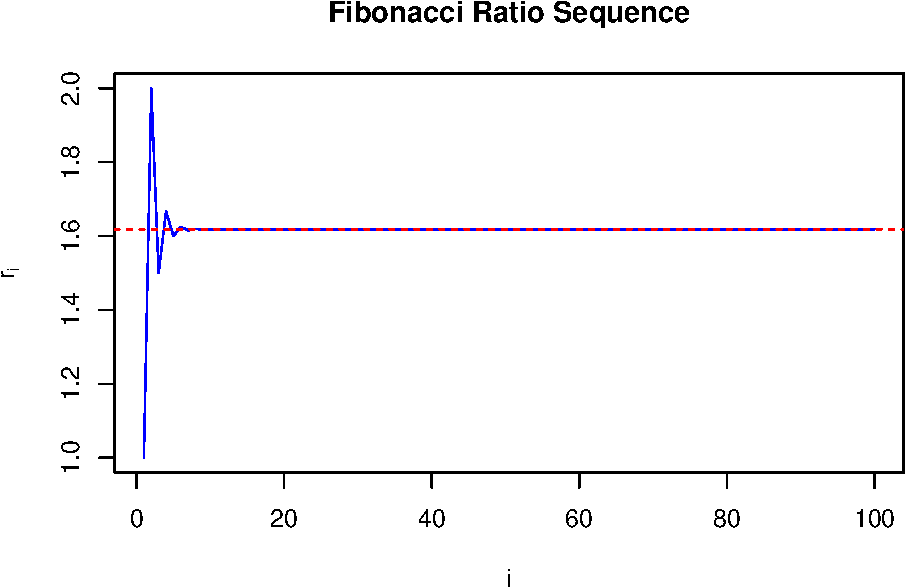
\includegraphics{CS1_files/figure-latex/unnamed-chunk-4-1.pdf} The ratio
\(r_i\) starts to stabilize around \(i = 20\). It converges to the
golden ratio:

\[
\frac{1 + \sqrt{5}}{2} \approx 1.618
\]

\section{2. Gamma function}\label{gamma-function}

\subsection{a.}\label{a.-1}

Write a function to compute the following for \(n\) a positive integer
using the \texttt{gamma} function in base R. \[
\rho_n =\frac{\Gamma((n-1)/2)}{\Gamma(1/2)\Gamma((n - 2)/2)}
\]

\begin{Shaded}
\begin{Highlighting}[]
\NormalTok{rho\_n }\OtherTok{\textless{}{-}} \ControlFlowTok{function}\NormalTok{(n) \{}
  \FunctionTok{gamma}\NormalTok{((n }\SpecialCharTok{{-}} \DecValTok{1}\NormalTok{) }\SpecialCharTok{/} \DecValTok{2}\NormalTok{) }\SpecialCharTok{/}\NormalTok{ (}\FunctionTok{gamma}\NormalTok{(}\DecValTok{1} \SpecialCharTok{/} \DecValTok{2}\NormalTok{) }\SpecialCharTok{*} \FunctionTok{gamma}\NormalTok{((n }\SpecialCharTok{{-}} \DecValTok{2}\NormalTok{) }\SpecialCharTok{/} \DecValTok{2}\NormalTok{))}
\NormalTok{\}}
\end{Highlighting}
\end{Shaded}

\subsection{b.}\label{b.-1}

Try \(n = 2000\). What do you observe? Why do you think the observed
behavior happens?

\begin{Shaded}
\begin{Highlighting}[]
\FunctionTok{rho\_n}\NormalTok{(}\DecValTok{2000}\NormalTok{)}
\end{Highlighting}
\end{Shaded}

\begin{verbatim}
## [1] NaN
\end{verbatim}

The result is \texttt{NaN} because of numerical overflow. The the Gamma
function grows very fast, and R can't handle such large values directly.

\subsection{c.}\label{c.-1}

Write an implementation which can also deal with large values of
\(n>1000\).

\begin{Shaded}
\begin{Highlighting}[]
\NormalTok{rho\_n\_stable }\OtherTok{\textless{}{-}} \ControlFlowTok{function}\NormalTok{(n) \{}
\NormalTok{  log\_rho }\OtherTok{\textless{}{-}} \FunctionTok{lgamma}\NormalTok{((n }\SpecialCharTok{{-}} \DecValTok{1}\NormalTok{) }\SpecialCharTok{/} \DecValTok{2}\NormalTok{) }\SpecialCharTok{{-}}\NormalTok{ (}\FunctionTok{lgamma}\NormalTok{(}\DecValTok{1} \SpecialCharTok{/} \DecValTok{2}\NormalTok{) }\SpecialCharTok{+} \FunctionTok{lgamma}\NormalTok{((n }\SpecialCharTok{{-}} \DecValTok{2}\NormalTok{) }\SpecialCharTok{/} \DecValTok{2}\NormalTok{))}
  \FunctionTok{exp}\NormalTok{(log\_rho)}
\NormalTok{\}}
\end{Highlighting}
\end{Shaded}

Now it works even for large \(n\):

\begin{Shaded}
\begin{Highlighting}[]
\FunctionTok{rho\_n\_stable}\NormalTok{(}\DecValTok{2000}\NormalTok{)}
\end{Highlighting}
\end{Shaded}

\begin{verbatim}
## [1] 17.83009
\end{verbatim}

\subsection{d.~}\label{d.}

Plot \(\rho_n/\sqrt{n}\) for different values of \(n\). Can you guess
the limit of \(\rho_n/\sqrt{n}\) for \(n \rightarrow\infty\)?

\begin{Shaded}
\begin{Highlighting}[]
\NormalTok{n\_vals }\OtherTok{\textless{}{-}} \DecValTok{1}\SpecialCharTok{:}\DecValTok{200}
\NormalTok{ratios }\OtherTok{\textless{}{-}} \FunctionTok{sapply}\NormalTok{(n\_vals, }\ControlFlowTok{function}\NormalTok{(n) }\FunctionTok{rho\_n\_stable}\NormalTok{(n) }\SpecialCharTok{/} \FunctionTok{sqrt}\NormalTok{(n))}

\FunctionTok{plot}\NormalTok{(n\_vals, ratios, }\AttributeTok{type =} \StringTok{"l"}\NormalTok{, }\AttributeTok{col =} \StringTok{"blue"}\NormalTok{, }\AttributeTok{lwd =} \DecValTok{2}\NormalTok{,}
     \AttributeTok{main =} \FunctionTok{expression}\NormalTok{(rho[n] }\SpecialCharTok{/} \FunctionTok{sqrt}\NormalTok{(n)),}
     \AttributeTok{xlab =} \StringTok{"n"}\NormalTok{, }\AttributeTok{ylab =} \FunctionTok{expression}\NormalTok{(rho[n] }\SpecialCharTok{/} \FunctionTok{sqrt}\NormalTok{(n)))}
\end{Highlighting}
\end{Shaded}

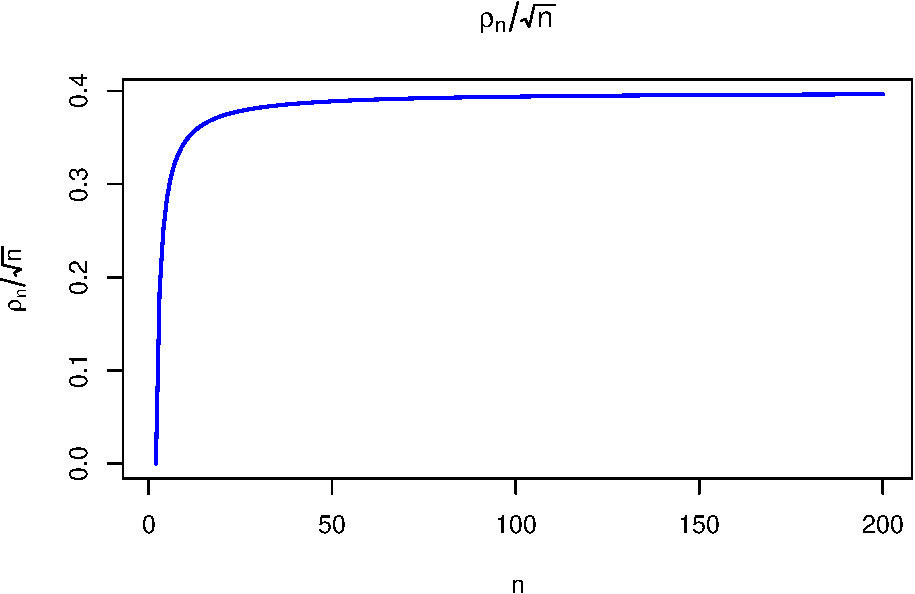
\includegraphics{CS1_files/figure-latex/unnamed-chunk-9-1.pdf}

The plot shows that \(\rho_n / \sqrt{n}\) converges to a constant as
\(n \to \infty\), which is consistent with asymptotic properties of the
Gamma function.

\section{3. Weak law of large numbers}\label{weak-law-of-large-numbers}

The law of large numbers states that if you repeat an experiment
independently a large number of times and average the result, what you
obtain should be close to the expected value. Formally, the weak law of
large numbers states that if \(X_1, X_2, \ldots X_n\) are independently
and identically distributed (iid) random variables with a finite
expected value \(E(X_i)=\mu<\infty\), then, for any \(\epsilon > 0\)
\(\lim_{n\rightarrow \infty} P(|\bar X_n-\mu|>\epsilon)=0\) where
\(\bar X_n=\frac{X_1+X_2+\ldots+X_n}{n}\) is the sample mean (the sample
mean converges in probability to the expected value).

\subsection{a.}\label{a.-2}

\begin{itemize}
\tightlist
\item
  In R, simulate rolling a fair 6-sided die \(n=10\,000\) times using
  vectorized functions.
\item
  After each roll, compute the cumulative mean of all previous rolls.
\end{itemize}

\begin{Shaded}
\begin{Highlighting}[]
\NormalTok{n }\OtherTok{\textless{}{-}} \DecValTok{10000}
\NormalTok{rolls }\OtherTok{\textless{}{-}} \FunctionTok{sample}\NormalTok{(}\DecValTok{1}\SpecialCharTok{:}\DecValTok{6}\NormalTok{, n, }\AttributeTok{replace =} \ConstantTok{TRUE}\NormalTok{)}
\NormalTok{running\_avg }\OtherTok{\textless{}{-}} \FunctionTok{cumsum}\NormalTok{(rolls) }\SpecialCharTok{/}\NormalTok{ (}\DecValTok{1}\SpecialCharTok{:}\NormalTok{n)}
\end{Highlighting}
\end{Shaded}

\begin{itemize}
\tightlist
\item
  Plot the running average against the number of rolls and comment on
  the result.
\end{itemize}

\begin{Shaded}
\begin{Highlighting}[]
\FunctionTok{plot}\NormalTok{(running\_avg, }\AttributeTok{type =} \StringTok{"l"}\NormalTok{, }\AttributeTok{col =} \StringTok{"blue"}\NormalTok{,}
     \AttributeTok{main =} \StringTok{"Running Average of 10,000 Dice Rolls"}\NormalTok{,}
     \AttributeTok{xlab =} \StringTok{"Number of Rolls"}\NormalTok{, }\AttributeTok{ylab =} \StringTok{"Running Average"}\NormalTok{)}
\FunctionTok{abline}\NormalTok{(}\AttributeTok{h =} \FloatTok{3.5}\NormalTok{, }\AttributeTok{col =} \StringTok{"red"}\NormalTok{, }\AttributeTok{lty =} \DecValTok{2}\NormalTok{)}
\end{Highlighting}
\end{Shaded}

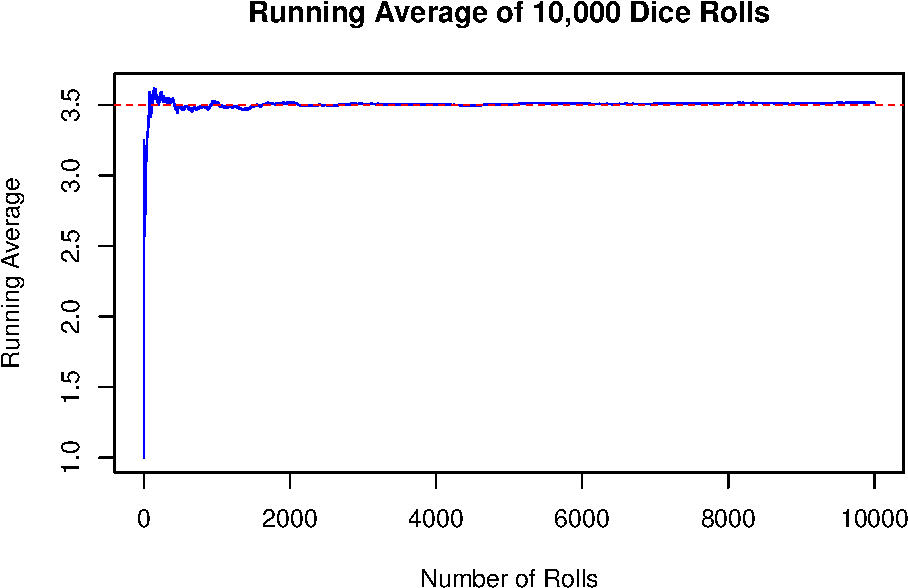
\includegraphics{CS1_files/figure-latex/unnamed-chunk-11-1.pdf} This
plot shows how the running average changes as we roll the die more
times. At the start, the average jumps around a lot because each new
roll has a big effect. But after a while, it starts to settle down.

After about 3000 rolls, it hardly changes anymore. This matches what the
Weak Law of Large Numbers says: the average of many die rolls should get
closer to the true mean (3.5).

\subsection{b.}\label{b.-2}

\begin{itemize}
\tightlist
\item
  Replicate the die-rolling experiment \(M=50\) times using a for loop.
  This will result in \(50\) paths which you can plot against the number
  of rolls.
\end{itemize}

\begin{Shaded}
\begin{Highlighting}[]
\NormalTok{M }\OtherTok{\textless{}{-}} \DecValTok{50}
\NormalTok{paths }\OtherTok{\textless{}{-}} \FunctionTok{matrix}\NormalTok{(}\ConstantTok{NA}\NormalTok{, }\AttributeTok{nrow =}\NormalTok{ n, }\AttributeTok{ncol =}\NormalTok{ M)}

\ControlFlowTok{for}\NormalTok{ (i }\ControlFlowTok{in} \DecValTok{1}\SpecialCharTok{:}\NormalTok{M) \{}
\NormalTok{  rolls }\OtherTok{\textless{}{-}} \FunctionTok{sample}\NormalTok{(}\DecValTok{1}\SpecialCharTok{:}\DecValTok{6}\NormalTok{, n, }\AttributeTok{replace =} \ConstantTok{TRUE}\NormalTok{)}
\NormalTok{  paths[, i] }\OtherTok{\textless{}{-}} \FunctionTok{cumsum}\NormalTok{(rolls) }\SpecialCharTok{/}\NormalTok{ (}\DecValTok{1}\SpecialCharTok{:}\NormalTok{n)}
\NormalTok{\}}
\end{Highlighting}
\end{Shaded}

\begin{itemize}
\tightlist
\item
  Plot all 50 paths on the same graph to observe the variation in the
  running averages.
\end{itemize}

\begin{Shaded}
\begin{Highlighting}[]
\FunctionTok{matplot}\NormalTok{(paths, }\AttributeTok{type =} \StringTok{"l"}\NormalTok{, }\AttributeTok{lty =} \DecValTok{1}\NormalTok{, }\AttributeTok{col =} \FunctionTok{rgb}\NormalTok{(}\DecValTok{0}\NormalTok{, }\DecValTok{0}\NormalTok{, }\DecValTok{1}\NormalTok{, }\FloatTok{0.2}\NormalTok{),}
        \AttributeTok{xlab =} \StringTok{"Number of Rolls"}\NormalTok{, }\AttributeTok{ylab =} \StringTok{"Running Average"}\NormalTok{,}
        \AttributeTok{main =} \StringTok{"50 Running Averages of Dice Rolls"}\NormalTok{)}
\FunctionTok{abline}\NormalTok{(}\AttributeTok{h =} \FloatTok{3.5}\NormalTok{, }\AttributeTok{col =} \StringTok{"red"}\NormalTok{, }\AttributeTok{lty =} \DecValTok{2}\NormalTok{)}
\end{Highlighting}
\end{Shaded}

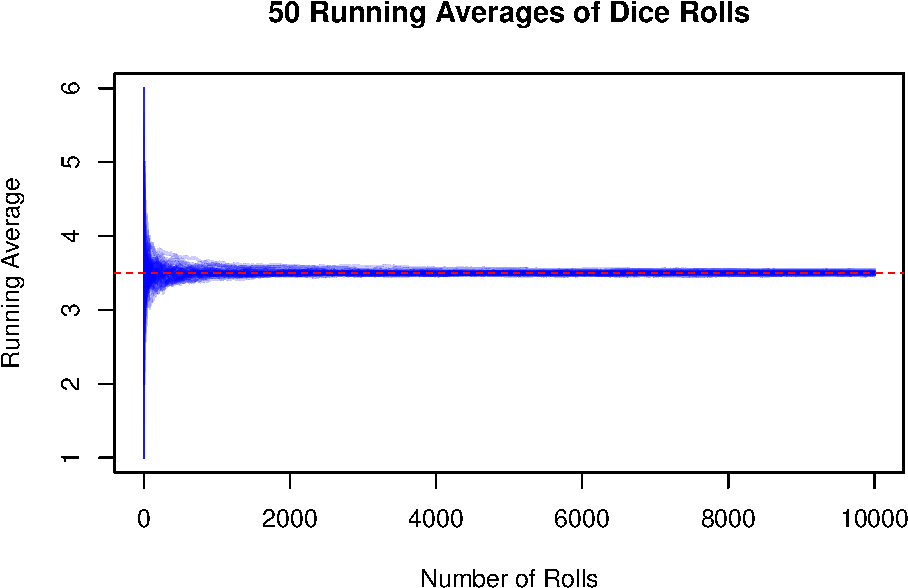
\includegraphics{CS1_files/figure-latex/unnamed-chunk-13-1.pdf} Each
line in this plot shows how the average of die rolls changes over time
for a single experiment. At the beginning, the paths are all over the
place because the average is very sensitive to the first few values. But
as more rolls are added, the averages become more stable and start to
cluster around 3.5.

By the end, almost all paths are very close to 3.5, which is exactly
what we expect from the Weak Law of Large Numbers. It shows that even
though each experiment is random, the average gets close to the expected
value when we repeat it enough times.

\subsection{c.}\label{c.-2}

What is the theoretical expected value of a fair 6-sided die?

The expected value \(\mu\) of a fair 6-sided die is: \[
\mu = \frac{1 + 2 + 3 + 4 + 5 + 6}{6} = 3.5
\]

\subsection{d.~}\label{d.-1}

Comment on how the running mean of the paths behaves relative to the
expected value as \(n\) increases.

As n approaches infinity, the running average converges to the expected
value 3.5, confirming the Weak Law of Large Numbers.

\subsection{e.}\label{e.}

\begin{itemize}
\item
  Modify the code in b. to use a while loop.
\item
  Stop the loop when the proportion of replications where the difference
  between the running average and the expected value lies outside the
  interval \([-\epsilon,\epsilon]\) is less than 0.05. Use
  \(\epsilon = 0.01\).
\item
  How high is \(n\) at the end of the loop?
\end{itemize}

\begin{Shaded}
\begin{Highlighting}[]
\NormalTok{epsilon }\OtherTok{\textless{}{-}} \FloatTok{0.01}
\NormalTok{max\_iter }\OtherTok{\textless{}{-}} \FloatTok{1e6}

\NormalTok{rolls\_matrix }\OtherTok{\textless{}{-}} \FunctionTok{matrix}\NormalTok{(}\FunctionTok{sample}\NormalTok{(}\DecValTok{1}\SpecialCharTok{:}\DecValTok{6}\NormalTok{, max\_iter }\SpecialCharTok{*}\NormalTok{ M, }\AttributeTok{replace =} \ConstantTok{TRUE}\NormalTok{), }\AttributeTok{nrow =}\NormalTok{ max\_iter, }\AttributeTok{ncol =}\NormalTok{ M)}
\NormalTok{running\_avg }\OtherTok{\textless{}{-}} \FunctionTok{matrix}\NormalTok{(}\ConstantTok{NA}\NormalTok{, }\AttributeTok{nrow =}\NormalTok{ max\_iter, }\AttributeTok{ncol =}\NormalTok{ M)}

\NormalTok{running\_avg[}\DecValTok{1}\NormalTok{, ] }\OtherTok{\textless{}{-}}\NormalTok{ rolls\_matrix[}\DecValTok{1}\NormalTok{, ]}
\NormalTok{j }\OtherTok{\textless{}{-}} \DecValTok{2}
\NormalTok{prop\_in }\OtherTok{\textless{}{-}} \DecValTok{0}

\ControlFlowTok{while}\NormalTok{ (j }\SpecialCharTok{\textless{}=}\NormalTok{ max\_iter }\SpecialCharTok{\&\&}\NormalTok{ prop\_in }\SpecialCharTok{\textless{}} \FloatTok{0.95}\NormalTok{) \{}
\NormalTok{  running\_avg[j, ] }\OtherTok{\textless{}{-}}\NormalTok{ (running\_avg[j }\SpecialCharTok{{-}} \DecValTok{1}\NormalTok{, ] }\SpecialCharTok{*}\NormalTok{ (j }\SpecialCharTok{{-}} \DecValTok{1}\NormalTok{) }\SpecialCharTok{+}\NormalTok{ rolls\_matrix[j, ]) }\SpecialCharTok{/}\NormalTok{ j}
\NormalTok{  prop\_in }\OtherTok{\textless{}{-}} \FunctionTok{mean}\NormalTok{(}\FunctionTok{abs}\NormalTok{(running\_avg[j, ] }\SpecialCharTok{{-}} \FloatTok{3.5}\NormalTok{) }\SpecialCharTok{\textless{}=}\NormalTok{ epsilon)}
\NormalTok{  j }\OtherTok{\textless{}{-}}\NormalTok{ j }\SpecialCharTok{+} \DecValTok{1}
\NormalTok{\}}

\FunctionTok{cat}\NormalTok{(}\StringTok{"Stopped at n ="}\NormalTok{, j }\SpecialCharTok{{-}} \DecValTok{1}\NormalTok{, }\StringTok{"with proportion in range:"}\NormalTok{, }\FunctionTok{round}\NormalTok{(prop\_in, }\DecValTok{3}\NormalTok{))}
\end{Highlighting}
\end{Shaded}

\begin{verbatim}
## Stopped at n = 79023 with proportion in range: 0.96
\end{verbatim}

\subsection{f.~}\label{f.}

\begin{itemize}
\tightlist
\item
  Repeat the analysis in b, but instead of simulating from a discrete
  uniform distribution, simulate from a continuous standard cauchy
  distribution using \texttt{rcauchy()}. The (standard) cauchy
  distribution arises from the ratio of two independent mean zero
  (standard) normally distributed random variables.
\end{itemize}

\begin{Shaded}
\begin{Highlighting}[]
\NormalTok{cauchy\_paths }\OtherTok{\textless{}{-}} \FunctionTok{matrix}\NormalTok{(}\ConstantTok{NA}\NormalTok{, }\AttributeTok{nrow =}\NormalTok{ n, }\AttributeTok{ncol =}\NormalTok{ M)}

\ControlFlowTok{for}\NormalTok{ (i }\ControlFlowTok{in} \DecValTok{1}\SpecialCharTok{:}\NormalTok{M) \{}
\NormalTok{  x }\OtherTok{\textless{}{-}} \FunctionTok{rcauchy}\NormalTok{(n)}
\NormalTok{  cauchy\_paths[, i] }\OtherTok{\textless{}{-}} \FunctionTok{cumsum}\NormalTok{(x) }\SpecialCharTok{/}\NormalTok{ (}\DecValTok{1}\SpecialCharTok{:}\NormalTok{n)}
\NormalTok{\}}
\end{Highlighting}
\end{Shaded}

\begin{itemize}
\tightlist
\item
  Plot the running mean against increasing \(n\). Comment on whether the
  weak Law of Large Numbers seems to hold for this distribution. Explain
  why or why not.
\end{itemize}

\begin{Shaded}
\begin{Highlighting}[]
\FunctionTok{matplot}\NormalTok{(cauchy\_paths, }\AttributeTok{type =} \StringTok{"l"}\NormalTok{, }\AttributeTok{lty =} \DecValTok{1}\NormalTok{, }\AttributeTok{col =} \FunctionTok{rgb}\NormalTok{(}\DecValTok{1}\NormalTok{, }\DecValTok{0}\NormalTok{, }\DecValTok{0}\NormalTok{, }\FloatTok{0.2}\NormalTok{),}
        \AttributeTok{main =} \StringTok{"Cauchy Running Averages"}\NormalTok{,}
        \AttributeTok{xlab =} \StringTok{"n"}\NormalTok{, }\AttributeTok{ylab =} \StringTok{"Running Mean"}\NormalTok{)}
\end{Highlighting}
\end{Shaded}

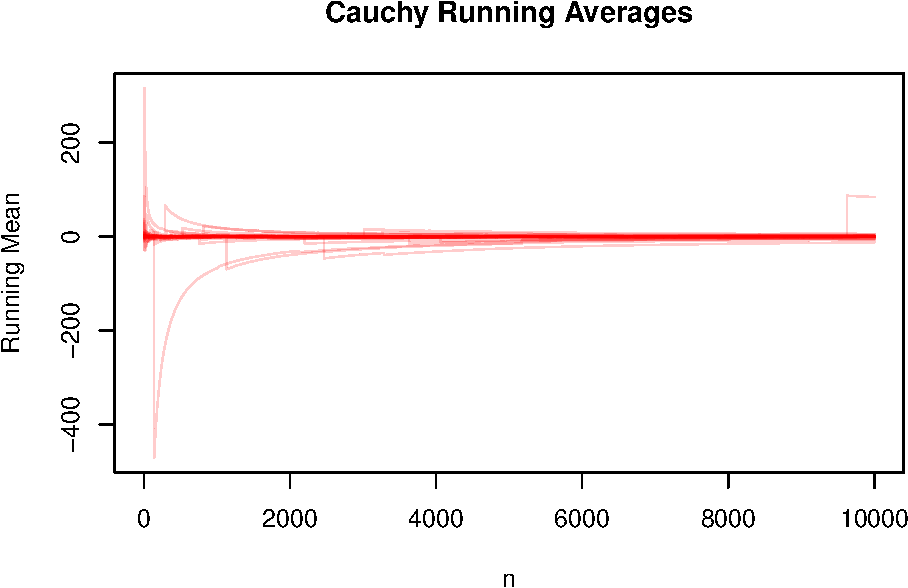
\includegraphics{CS1_files/figure-latex/unnamed-chunk-16-1.pdf}

This plot shows the running averages for 50 simulations of
Cauchy-distributed random variables. Unlike the die rolls, these paths
don't settle down or stabilize around a specific value. Some paths shoot
up or down dramatically even after thousands of iterations.

This happens because the Cauchy distribution doesn't have a defined mean
or variance. So the Law of Large Numbers doesn't apply here. The average
doesn't converge like it did with the uniform distribution of the die
rolls. Instead, it stays unstable, and a few extreme values can heavily
influence the result even with many observations.

\section{4. Central limit theorem}\label{central-limit-theorem}

The central limit theorem states that, under certain conditions, the sum
of a large number of random variables is approximately normal. Consider
the case where \(X_1, X_2,\ldots,X_n\) are i.i.d. random variables with
finite expected values (\(E(X_i)=\mu<\infty\)) and variances
\((Var(X_i)=\sigma^2<\infty)\). The central limit theorem states that
the cumulative distribution function (CDF) of the normalized random
variable \[
Z_n = \frac{\bar X_n - \mu}{\sigma/\sqrt{n}}
\] converges to the standard normal CDF as \(n\rightarrow\infty\).

\subsection{a.}\label{a.-3}

Derive the expected value of the sample mean
\(\bar X_n=\frac{X_1+X_2+\ldots+X_n}{n}\).

Let \(X_1, X_2, \ldots, X_n\) be i.i.d. random variables with expected
value \(\mu = E[X_i]\).

The sample mean is defined as:

\[
\bar{X}_n = \frac{1}{n} \sum_{i=1}^n X_i
\]

To find the expected value of \(\bar{X}_n\), we use the linearity of
expectation:

\[
E[\bar{X}_n] = E\left[ \frac{1}{n} \sum_{i=1}^n X_i \right]
= \frac{1}{n} \sum_{i=1}^n E[X_i]
= \frac{1}{n} \cdot n \cdot \mu = \mu
\]

So, the expected value of the sample mean is equal to the population
mean: \[
E[\bar{X}_n] = \mu
\]

\subsection{b.}\label{b.-3}

Derive the variance of the sample mean
\(\bar X_n=\frac{X_1+X_2+\ldots+X_n}{n}\).

Let \(\sigma^2 = \text{Var}(X_i)\). Since the \(X_i\) are i.i.d., the
variance of the sample mean is:

\[
\text{Var}(\bar{X}_n) = \text{Var}\left( \frac{1}{n} \sum_{i=1}^n X_i \right)
\]

We use the rule that \(\text{Var}(aX) = a^2 \cdot \text{Var}(X)\) and
the independence of the \(X_i\):

\[
\text{Var}(\bar{X}_n) = \frac{1}{n^2} \sum_{i=1}^n \text{Var}(X_i)
= \frac{1}{n^2} \cdot n \cdot \sigma^2 = \frac{\sigma^2}{n}
\]

So, the variance of the sample mean decreases with \(n\): \[
\text{Var}(\bar{X}_n) = \frac{\sigma^2}{n}
\]

\subsection{c.~}\label{c.-3}

The central limit theorem makes few assumption on the distribution of
the random variables \(X_i\). Consider again the die-rolling experiment
where \(X_i\) is the random variable giving the number in roll \(i\).

\begin{itemize}
\item
  Simulate Die Rolls: For each value of \(n\) (where
  \(n=\{100,1000,10000\}\)), simulate rolling a die \(n\) times. Record
  the mean of the \(n\) rolls.
\item
  Repeat the above process \(M=100\) times for each value of \(n\). This
  will give you 100 sample means for each \(n\).
\end{itemize}

\begin{Shaded}
\begin{Highlighting}[]
\NormalTok{get\_means }\OtherTok{\textless{}{-}} \ControlFlowTok{function}\NormalTok{(n, M) \{}
  \FunctionTok{replicate}\NormalTok{(M, }\FunctionTok{mean}\NormalTok{(}\FunctionTok{sample}\NormalTok{(}\DecValTok{1}\SpecialCharTok{:}\DecValTok{6}\NormalTok{, n, }\AttributeTok{replace =} \ConstantTok{TRUE}\NormalTok{)))}
\NormalTok{\}}

\NormalTok{means\_100 }\OtherTok{\textless{}{-}} \FunctionTok{get\_means}\NormalTok{(}\DecValTok{100}\NormalTok{, }\DecValTok{100}\NormalTok{)}
\NormalTok{means\_1000 }\OtherTok{\textless{}{-}} \FunctionTok{get\_means}\NormalTok{(}\DecValTok{1000}\NormalTok{, }\DecValTok{100}\NormalTok{)}
\NormalTok{means\_10000 }\OtherTok{\textless{}{-}} \FunctionTok{get\_means}\NormalTok{(}\DecValTok{10000}\NormalTok{, }\DecValTok{100}\NormalTok{)}
\end{Highlighting}
\end{Shaded}

\begin{itemize}
\tightlist
\item
  Plot a histogram of the 100 sample means for each value of \(n\).
  Observe the shape of the histograms.
\end{itemize}

\begin{Shaded}
\begin{Highlighting}[]
\NormalTok{x\_limits }\OtherTok{\textless{}{-}} \FunctionTok{range}\NormalTok{(}\FunctionTok{c}\NormalTok{(means\_100, means\_1000, means\_10000))}

\FunctionTok{par}\NormalTok{(}\AttributeTok{mfrow =} \FunctionTok{c}\NormalTok{(}\DecValTok{1}\NormalTok{, }\DecValTok{3}\NormalTok{))}
\FunctionTok{hist}\NormalTok{(means\_100, }\AttributeTok{main =} \StringTok{"n = 100"}\NormalTok{, }\AttributeTok{xlab =} \StringTok{"Sample Mean"}\NormalTok{, }\AttributeTok{col =} \StringTok{"lightblue"}\NormalTok{,}
     \AttributeTok{breaks =} \DecValTok{20}\NormalTok{, }\AttributeTok{xlim =}\NormalTok{ x\_limits)}
\FunctionTok{hist}\NormalTok{(means\_1000, }\AttributeTok{main =} \StringTok{"n = 1000"}\NormalTok{, }\AttributeTok{xlab =} \StringTok{"Sample Mean"}\NormalTok{, }\AttributeTok{col =} \StringTok{"lightgreen"}\NormalTok{,}
     \AttributeTok{breaks =} \DecValTok{20}\NormalTok{, }\AttributeTok{xlim =}\NormalTok{ x\_limits)}
\FunctionTok{hist}\NormalTok{(means\_10000, }\AttributeTok{main =} \StringTok{"n = 10000"}\NormalTok{, }\AttributeTok{xlab =} \StringTok{"Sample Mean"}\NormalTok{, }\AttributeTok{col =} \StringTok{"lightpink"}\NormalTok{,}
     \AttributeTok{breaks =} \DecValTok{20}\NormalTok{, }\AttributeTok{xlim =}\NormalTok{ x\_limits)}
\end{Highlighting}
\end{Shaded}

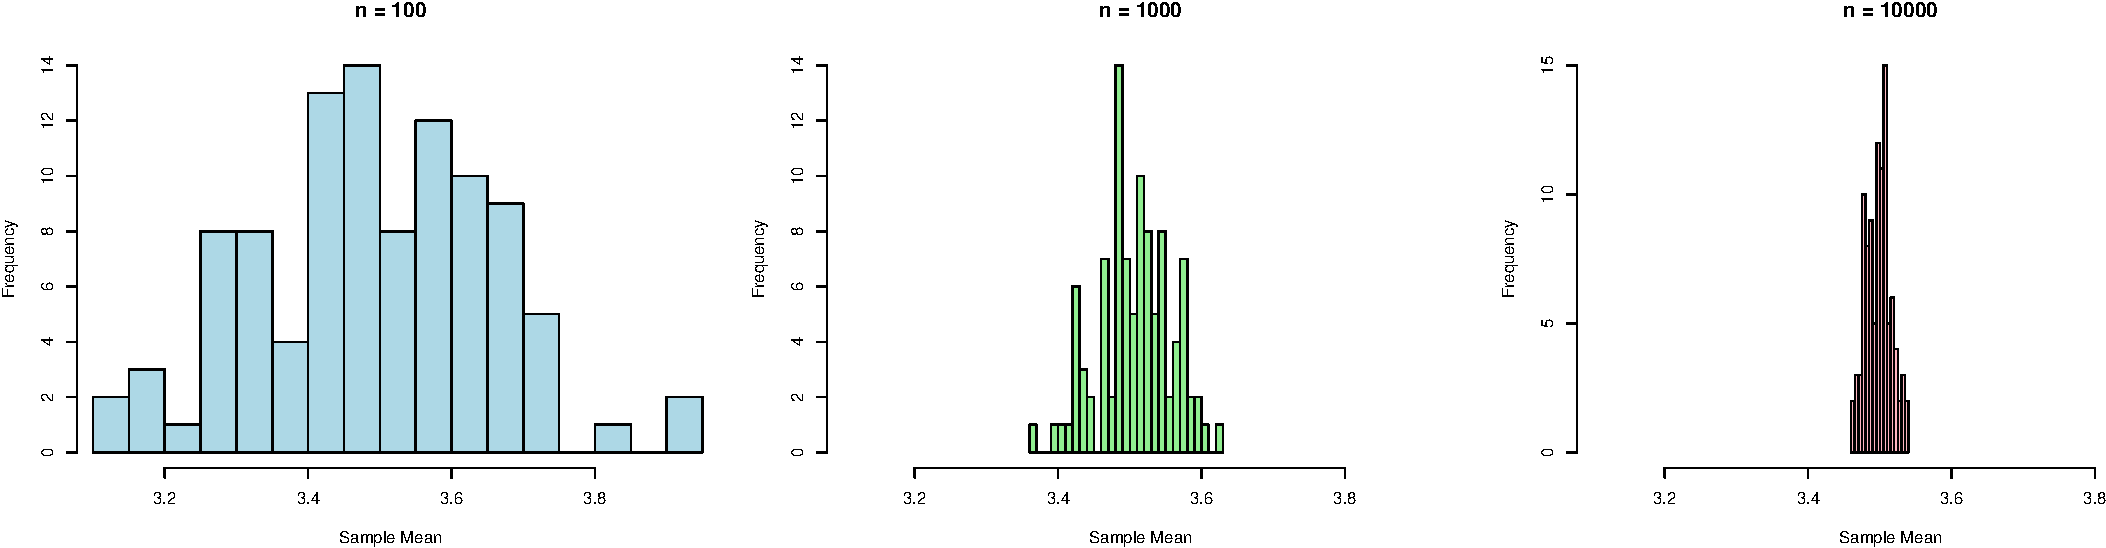
\includegraphics{CS1_files/figure-latex/unnamed-chunk-18-1.pdf}

\begin{itemize}
\tightlist
\item
  Discuss how the distribution of the sample means changes as \(n\)
  increases. Comment on whether the histograms appear to approach a
  normal distribution as \(n\), illustrating the Central Limit Theorem.
\end{itemize}

The distribution of the sample means changes as the number of die rolls
\(n\) increases:

\begin{itemize}
\item
  \textbf{When \(n = 100\):} The sample means are spread out and the
  shape is a bit uneven. There's still a lot of variation, but the
  values seem to center around 3.5.
\item
  \textbf{When \(n = 1000\):} The distribution is narrower and looks
  more symmetric. The sample means are more tightly grouped, and it
  already starts to look like a normal distribution.
\item
  \textbf{When \(n = 10000\):} The histogram is very concentrated around
  the mean of 3.5, and the shape looks almost perfectly normal.
\end{itemize}

As \(n\) gets larger, the sample means become less variable and more
normally distributed. Even though we're rolling a fair die (which gives
discrete uniform outcomes), the average of many rolls behaves like it's
coming from a normal distribution when we repeat the experiment enough
times.

\subsection{d.~}\label{d.-2}

Compute expected value \(\mu\) and the variance \(\sigma^2\) for the
random variable \(X_i\) (giving the number in die-roll \(i\)), which
follows a discrete uniform distribution.

The possible outcomes are \(\{1, 2, 3, 4, 5, 6\}\), each with equal
probability \(\frac{1}{6}\).

\paragraph{\texorpdfstring{Expected Value
\(\mu\):}{Expected Value \textbackslash mu:}}\label{expected-value-mu}

\[
\mu = \frac{1 + 2 + 3 + 4 + 5 + 6}{6} = \frac{21}{6} = 3.5
\]

\paragraph{\texorpdfstring{Variance
\(\sigma^2\):}{Variance \textbackslash sigma\^{}2:}}\label{variance-sigma2}

\[
\sigma^2 = \frac{1}{6} \sum_{i=1}^{6} (i - 3.5)^2 = \frac{(6.25 + 2.25 + 0.25 + 0.25 + 2.25 + 6.25)}{6} = \frac{17.5}{6} = \frac{35}{12} \approx 2.9167
\]

So the theoretical values are:

\begin{itemize}
\tightlist
\item
  \(\mu = 3.5\)
\item
  \(\sigma^2 = \frac{35}{12} \approx 2.9167\)
\end{itemize}

\subsection{e.}\label{e.-1}

Now that you computed \(\mu\) and \(\sigma^2\), consider \(Z_n\).

\begin{itemize}
\tightlist
\item
  For each value of \(n\) (where \(n=\{100,1000,10000\}\)) and for
  \(M=\{100,1000,10000\}\) replications, simulate the rolling of \(n\)
  dice and calculate the \(Z_n\).
\end{itemize}

\begin{Shaded}
\begin{Highlighting}[]
\NormalTok{simulate\_Zn }\OtherTok{\textless{}{-}} \ControlFlowTok{function}\NormalTok{(n, M, }\AttributeTok{mu =} \FloatTok{3.5}\NormalTok{, }\AttributeTok{sigma =} \FunctionTok{sqrt}\NormalTok{(}\DecValTok{35}\SpecialCharTok{/}\DecValTok{12}\NormalTok{)) \{}
  \FunctionTok{replicate}\NormalTok{(M, \{}
\NormalTok{    x }\OtherTok{\textless{}{-}} \FunctionTok{sample}\NormalTok{(}\DecValTok{1}\SpecialCharTok{:}\DecValTok{6}\NormalTok{, n, }\AttributeTok{replace =} \ConstantTok{TRUE}\NormalTok{)}
\NormalTok{    (}\FunctionTok{mean}\NormalTok{(x) }\SpecialCharTok{{-}}\NormalTok{ mu) }\SpecialCharTok{/}\NormalTok{ (sigma }\SpecialCharTok{/} \FunctionTok{sqrt}\NormalTok{(n))}
\NormalTok{  \})}
\NormalTok{\}}

\NormalTok{Z\_data }\OtherTok{\textless{}{-}} \FunctionTok{list}\NormalTok{(}
  \StringTok{"n=100\_M=100"} \OtherTok{=} \FunctionTok{simulate\_Zn}\NormalTok{(}\DecValTok{100}\NormalTok{, }\DecValTok{100}\NormalTok{),}
  \StringTok{"n=1000\_M=100"} \OtherTok{=} \FunctionTok{simulate\_Zn}\NormalTok{(}\DecValTok{1000}\NormalTok{, }\DecValTok{100}\NormalTok{),}
  \StringTok{"n=10000\_M=100"} \OtherTok{=} \FunctionTok{simulate\_Zn}\NormalTok{(}\DecValTok{10000}\NormalTok{, }\DecValTok{100}\NormalTok{),}
  \StringTok{"n=1000\_M=1000"} \OtherTok{=} \FunctionTok{simulate\_Zn}\NormalTok{(}\DecValTok{1000}\NormalTok{, }\DecValTok{1000}\NormalTok{),}
  \StringTok{"n=10000\_M=10000"} \OtherTok{=} \FunctionTok{simulate\_Zn}\NormalTok{(}\DecValTok{10000}\NormalTok{, }\DecValTok{10000}\NormalTok{)}
\NormalTok{)}
\end{Highlighting}
\end{Shaded}

\begin{itemize}
\tightlist
\item
  Plot histograms of \(Z_n\) for each combination of \(n\) and \(M\).
\end{itemize}

\begin{Shaded}
\begin{Highlighting}[]
\FunctionTok{par}\NormalTok{(}\AttributeTok{mfrow =} \FunctionTok{c}\NormalTok{(}\DecValTok{2}\NormalTok{, }\DecValTok{3}\NormalTok{))}
\ControlFlowTok{for}\NormalTok{ (name }\ControlFlowTok{in} \FunctionTok{names}\NormalTok{(Z\_data)) \{}
  \FunctionTok{hist}\NormalTok{(Z\_data[[name]], }\AttributeTok{main =}\NormalTok{ name, }\AttributeTok{xlab =} \StringTok{"Zn"}\NormalTok{, }\AttributeTok{breaks =} \DecValTok{20}\NormalTok{, }\AttributeTok{col =} \StringTok{"skyblue"}\NormalTok{)}
\NormalTok{\}}
\end{Highlighting}
\end{Shaded}

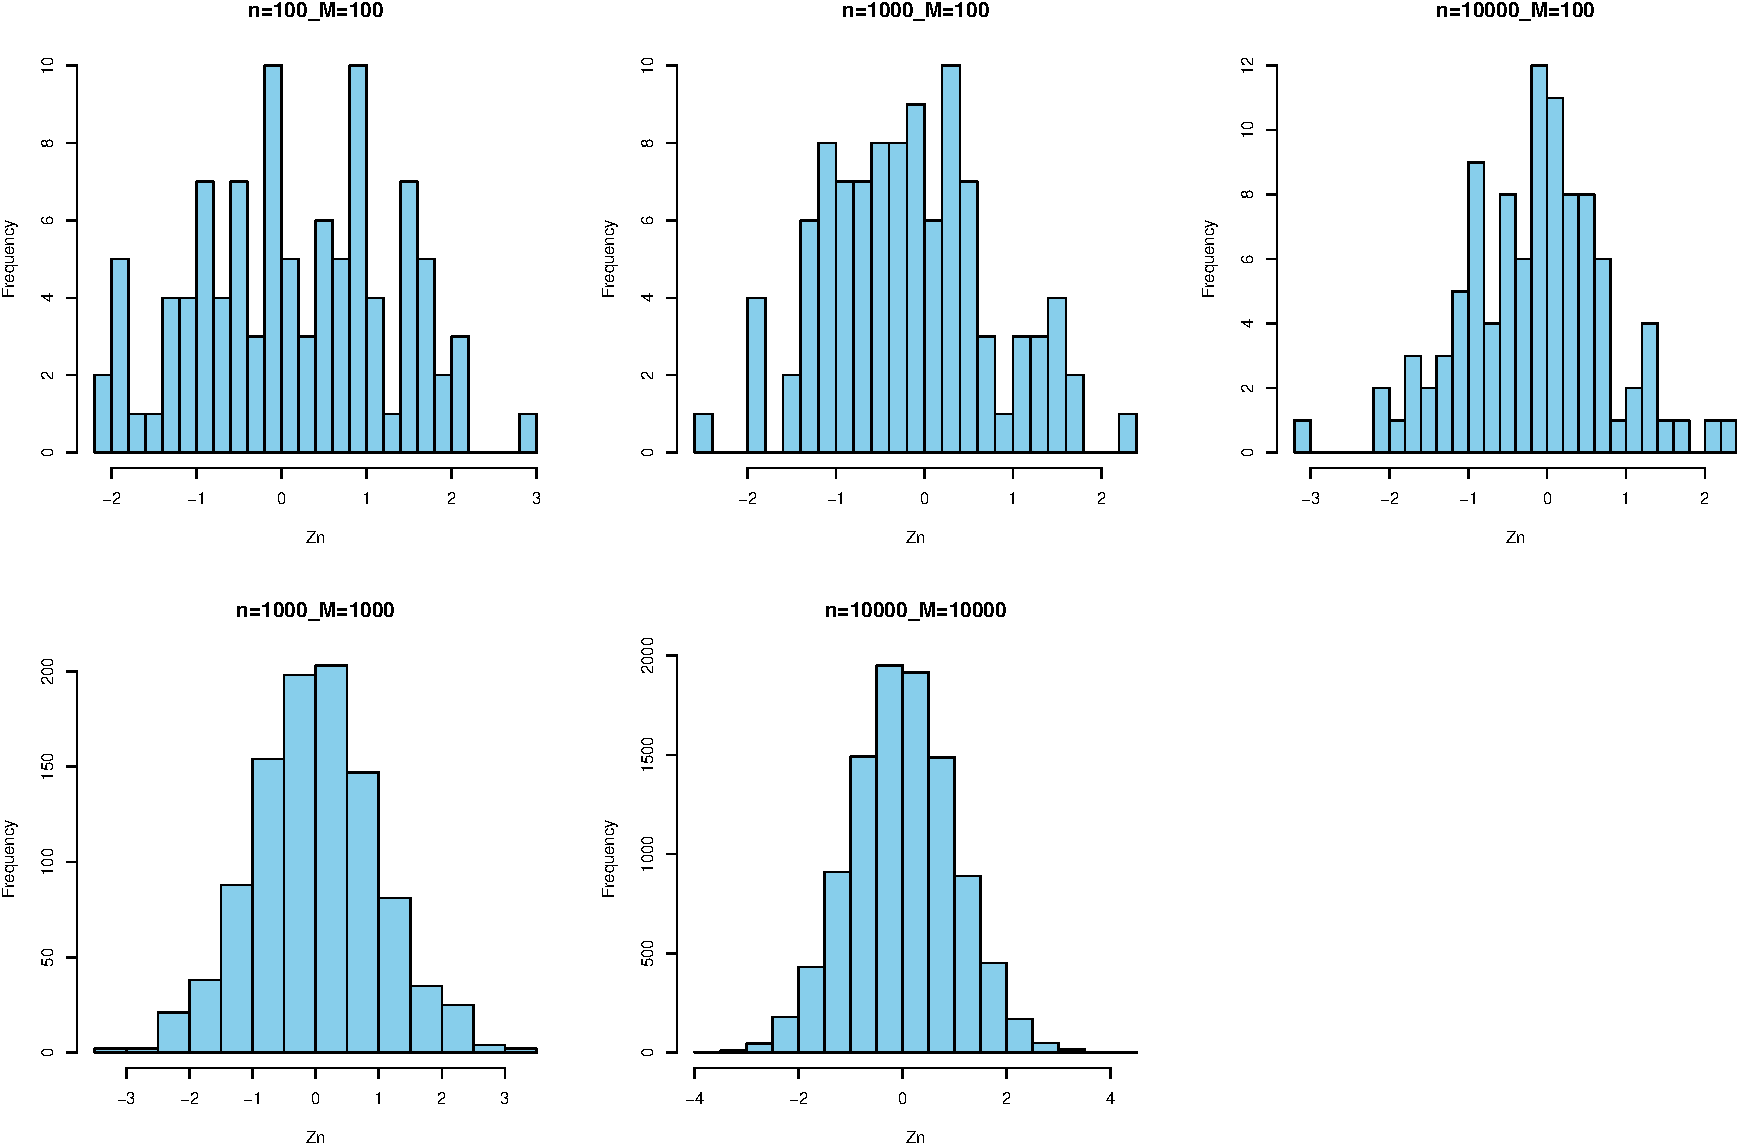
\includegraphics{CS1_files/figure-latex/unnamed-chunk-20-1.pdf}

\begin{itemize}
\tightlist
\item
  Discuss how the distribution of \(Z_n\) changes as \(n\) and \(M\)
  increase. Comment on whether the distributions of \(Z_n\) appear to
  approach a normal distribution, illustrating the Central Limit
  Theorem.
\end{itemize}

Recall that:

\[
Z_n = \frac{\bar{X}_n - \mu}{\sigma / \sqrt{n}}
\]

\textbf{Effect of \(n\):}

As \emph{n} increases:

\begin{itemize}
\tightlist
\item
  The sample mean \(\bar{X}_n\) becomes more concentrated around the
  true mean \(\mu\).
\item
  So \(Z_n\) becomes less variable, and its distribution gets tighter
  and more normal-shaped.
\item
  You can clearly see that in the bottom row (large \emph{n}), where the
  histograms are symmetric and bell-shaped.
\end{itemize}

\textbf{Effect of \(M\):}

\emph{M} controls how many values of \(Z_n\) you generate.

As \emph{M} increases:

\begin{itemize}
\tightlist
\item
  The histogram becomes smoother and more accurate, because you have
  more data points.
\item
  It doesn't change the distribution's shape but makes it easier to see
  the bell curve.
\item
  Compare the rough, jagged histograms when \emph{M = 100} (top row)
  with the very smooth ones when \emph{M = 10000} (bottom middle).
\end{itemize}

From the histograms, the distribution of \(Z_n\) becomes more
``normal-looking'' as both the sample size \(n\) and the number of
replications \(M\) increase. When \(M = 100\), the distributions are
still a bit uneven and noisy, even if \(n\) is large. This is likely
because 100 repetitions aren't enough to fully capture the shape of the
distribution.

As \(M\) increases to 1000 and 10000, the histograms get much smoother
and start to show the bell-shaped curve we expect from a standard normal
distribution.

Increasing \(n\) makes each \(Z_n\) more stable. With larger \(n\), the
standardized means are less variable and cluster more tightly around 0.

Overall, the results clearly show the \textbf{Central Limit Theorem}:\\
The distribution of the standardized sample mean \(Z_n\) approaches the
standard normal distribution as \(n\) and \(M\) increase --- even though
the original data (rolling a fair die) comes from a discrete, non-normal
distribution.

\section{5. Readable and efficient
code}\label{readable-and-efficient-code}

Read over the code below.

\subsection{a.}\label{a.-4}

Explain (in text) what the code does.

This function generates 100 random values from a normal distribution
using the rnorm() function for variables x and z. Afterwards it checks
if a threshold for the sum of the x values are met. If not, the
execution is stopped. Then it goes on to fit a linear model using these
variables. It also takes the sine function of the residuals and adds a
bit of noise to create the next value of x. This is repeated 4 times. At
the end a dataframe is created based on the x and newly created y
values, which are based on x and some noise.

In the second part of the function - a manual cross validation error
estimation is calculated. The function is parted in 4 sections - 1:250,
251:500, 501:750, and 751:1000. On all of these 4 parts, the linear
model is fit, predicted and the root mean squared error is calculated.
The result is a vector of total 4 RMSE values of each of these 4 chunks.

\subsection{b.}\label{b.-4}

Explain (in text) what you would change to make the code more readable.

To make the code more readable, simple coding practices could make it
better. For example, adding comments to explain what part of the code is
responsible for what action (or what is intended by writing such and
such code). Secondly, adding meaningful variable names - instead of
x,y,z, we could write predictor, response and residuals. Thirdly, a lot
of the code is repetitive. Instead of writing the same code over and
over, we could wrap the code in a function to make our work more
efficient. Lastly, the code is just one big chunk of code - adding
spaces and lines to separate different part of the code would also make
it more clearer and easier to understand.

\subsection{c.}\label{c.-4}

Change the code according to b. and wrap it in a function. This function
should have at most 10 lines (without adding commands to more lines such
as \texttt{x\ \textless{}-\ 1;\ y\ \textless{}-\ 2}. Such commands will
count as 2 lines!). Check that the function called on the same input
outputs the same as the provided code.

\begin{Shaded}
\begin{Highlighting}[]
\FunctionTok{set.seed}\NormalTok{(}\DecValTok{1}\NormalTok{)}
\NormalTok{x }\OtherTok{\textless{}{-}} \FunctionTok{rnorm}\NormalTok{(}\DecValTok{100}\NormalTok{)}
\NormalTok{z }\OtherTok{\textless{}{-}} \FunctionTok{rnorm}\NormalTok{(}\DecValTok{100}\NormalTok{)}
\ControlFlowTok{if}\NormalTok{ (}\FunctionTok{sum}\NormalTok{(x }\SpecialCharTok{\textgreater{}=}\NormalTok{ .}\DecValTok{001}\NormalTok{) }\SpecialCharTok{\textless{}} \DecValTok{1}\NormalTok{) \{}
  \FunctionTok{stop}\NormalTok{(}\StringTok{"step 1 requires 1 observation(s) with value \textgreater{}= .001"}\NormalTok{)}
\NormalTok{\}}
\NormalTok{fit }\OtherTok{\textless{}{-}} \FunctionTok{lm}\NormalTok{(x }\SpecialCharTok{\textasciitilde{}}\NormalTok{ z)}
\NormalTok{r }\OtherTok{\textless{}{-}}\NormalTok{ fit}\SpecialCharTok{$}\NormalTok{residuals}
\NormalTok{x }\OtherTok{\textless{}{-}} \FunctionTok{sin}\NormalTok{(r) }\SpecialCharTok{+}\NormalTok{ .}\DecValTok{01}
\ControlFlowTok{if}\NormalTok{ (}\FunctionTok{sum}\NormalTok{(x }\SpecialCharTok{\textgreater{}=}\NormalTok{ .}\DecValTok{002}\NormalTok{) }\SpecialCharTok{\textless{}} \DecValTok{2}\NormalTok{) \{}
  \FunctionTok{stop}\NormalTok{(}\StringTok{"step 2 requires 2 observation(s) with value \textgreater{}= .002"}\NormalTok{)}
\NormalTok{\}}
\NormalTok{fit }\OtherTok{\textless{}{-}} \FunctionTok{lm}\NormalTok{(x }\SpecialCharTok{\textasciitilde{}}\NormalTok{ z)}
\NormalTok{r }\OtherTok{\textless{}{-}}\NormalTok{ fit}\SpecialCharTok{$}\NormalTok{residuals}
\NormalTok{x }\OtherTok{\textless{}{-}} \DecValTok{2} \SpecialCharTok{*} \FunctionTok{sin}\NormalTok{(r) }\SpecialCharTok{+}\NormalTok{ .}\DecValTok{02}
\ControlFlowTok{if}\NormalTok{ (}\FunctionTok{sum}\NormalTok{(x }\SpecialCharTok{\textgreater{}=}\NormalTok{ .}\DecValTok{003}\NormalTok{) }\SpecialCharTok{\textless{}} \DecValTok{3}\NormalTok{) \{}
  \FunctionTok{stop}\NormalTok{(}\StringTok{"step 3 requires 3 observation(s) with value \textgreater{}= .003"}\NormalTok{)}
\NormalTok{\}}
\NormalTok{fit }\OtherTok{\textless{}{-}} \FunctionTok{lm}\NormalTok{(x }\SpecialCharTok{\textasciitilde{}}\NormalTok{ z)}
\NormalTok{r }\OtherTok{\textless{}{-}}\NormalTok{ fit}\SpecialCharTok{$}\NormalTok{residuals}
\NormalTok{x }\OtherTok{\textless{}{-}} \DecValTok{3} \SpecialCharTok{*} \FunctionTok{sin}\NormalTok{(r) }\SpecialCharTok{+}\NormalTok{ .}\DecValTok{03}
\ControlFlowTok{if}\NormalTok{ (}\FunctionTok{sum}\NormalTok{(x }\SpecialCharTok{\textgreater{}=}\NormalTok{ .}\DecValTok{004}\NormalTok{) }\SpecialCharTok{\textless{}} \DecValTok{4}\NormalTok{) \{}
  \FunctionTok{stop}\NormalTok{(}\StringTok{"step 4 requires 4 observation(s) with value \textgreater{}= .004"}\NormalTok{)}
\NormalTok{\}}
\NormalTok{fit }\OtherTok{\textless{}{-}} \FunctionTok{lm}\NormalTok{(x }\SpecialCharTok{\textasciitilde{}}\NormalTok{ z)}
\NormalTok{r }\OtherTok{\textless{}{-}}\NormalTok{ fit}\SpecialCharTok{$}\NormalTok{residuals}
\NormalTok{x }\OtherTok{\textless{}{-}} \DecValTok{4} \SpecialCharTok{*} \FunctionTok{sin}\NormalTok{(r) }\SpecialCharTok{+}\NormalTok{ .}\DecValTok{04}
\NormalTok{x}
\end{Highlighting}
\end{Shaded}

\begin{Shaded}
\begin{Highlighting}[]
\FunctionTok{set.seed}\NormalTok{(}\DecValTok{1}\NormalTok{) }
\NormalTok{x }\OtherTok{\textless{}{-}} \FunctionTok{rnorm}\NormalTok{(}\DecValTok{1000}\NormalTok{)}
\NormalTok{y }\OtherTok{\textless{}{-}} \DecValTok{2} \SpecialCharTok{+}\NormalTok{ x }\SpecialCharTok{+} \FunctionTok{rnorm}\NormalTok{(}\DecValTok{1000}\NormalTok{)}
\NormalTok{df }\OtherTok{\textless{}{-}} \FunctionTok{data.frame}\NormalTok{(x, y)}

\FunctionTok{cat}\NormalTok{(}\StringTok{"Step"}\NormalTok{, }\DecValTok{1}\NormalTok{, }\StringTok{"}\SpecialCharTok{\textbackslash{}n}\StringTok{"}\NormalTok{)}
\NormalTok{fit1 }\OtherTok{\textless{}{-}} \FunctionTok{lm}\NormalTok{(y }\SpecialCharTok{\textasciitilde{}}\NormalTok{ x, }\AttributeTok{data =}\NormalTok{ df[}\SpecialCharTok{{-}}\NormalTok{(}\DecValTok{1}\SpecialCharTok{:}\DecValTok{250}\NormalTok{),])}
\NormalTok{p1 }\OtherTok{\textless{}{-}} \FunctionTok{predict}\NormalTok{(fit1, }\AttributeTok{newdata =}\NormalTok{ df[(}\DecValTok{1}\SpecialCharTok{:}\DecValTok{250}\NormalTok{),])}
\NormalTok{r }\OtherTok{\textless{}{-}} \FunctionTok{sqrt}\NormalTok{(}\FunctionTok{mean}\NormalTok{((p1 }\SpecialCharTok{{-}}\NormalTok{ df[(}\DecValTok{1}\SpecialCharTok{:}\DecValTok{250}\NormalTok{),}\StringTok{"y"}\NormalTok{])}\SpecialCharTok{\^{}}\DecValTok{2}\NormalTok{))  }

\FunctionTok{cat}\NormalTok{(}\StringTok{"Step"}\NormalTok{, }\DecValTok{2}\NormalTok{, }\StringTok{"}\SpecialCharTok{\textbackslash{}n}\StringTok{"}\NormalTok{)}
\NormalTok{fit2 }\OtherTok{\textless{}{-}} \FunctionTok{lm}\NormalTok{(y }\SpecialCharTok{\textasciitilde{}}\NormalTok{ x, }\AttributeTok{data =}\NormalTok{ df[}\SpecialCharTok{{-}}\NormalTok{(}\DecValTok{251}\SpecialCharTok{:}\DecValTok{500}\NormalTok{),])}
\NormalTok{p2 }\OtherTok{\textless{}{-}} \FunctionTok{predict}\NormalTok{(fit2, }\AttributeTok{newdata =}\NormalTok{ df[(}\DecValTok{251}\SpecialCharTok{:}\DecValTok{500}\NormalTok{),])}
\NormalTok{r }\OtherTok{\textless{}{-}} \FunctionTok{c}\NormalTok{(r, }\FunctionTok{sqrt}\NormalTok{(}\FunctionTok{mean}\NormalTok{((p2 }\SpecialCharTok{{-}}\NormalTok{ df[(}\DecValTok{251}\SpecialCharTok{:}\DecValTok{500}\NormalTok{),}\StringTok{"y"}\NormalTok{])}\SpecialCharTok{\^{}}\DecValTok{2}\NormalTok{)))}

\FunctionTok{cat}\NormalTok{(}\StringTok{"Step"}\NormalTok{, }\DecValTok{3}\NormalTok{, }\StringTok{"}\SpecialCharTok{\textbackslash{}n}\StringTok{"}\NormalTok{)}
\NormalTok{fit3 }\OtherTok{\textless{}{-}} \FunctionTok{lm}\NormalTok{(y }\SpecialCharTok{\textasciitilde{}}\NormalTok{ x, }\AttributeTok{data =}\NormalTok{ df[}\SpecialCharTok{{-}}\NormalTok{(}\DecValTok{501}\SpecialCharTok{:}\DecValTok{750}\NormalTok{),])}
\NormalTok{p3 }\OtherTok{\textless{}{-}} \FunctionTok{predict}\NormalTok{(fit3, }\AttributeTok{newdata =}\NormalTok{ df[(}\DecValTok{501}\SpecialCharTok{:}\DecValTok{750}\NormalTok{),])}
\NormalTok{r }\OtherTok{\textless{}{-}} \FunctionTok{c}\NormalTok{(r, }\FunctionTok{sqrt}\NormalTok{(}\FunctionTok{mean}\NormalTok{((p3 }\SpecialCharTok{{-}}\NormalTok{ df[(}\DecValTok{501}\SpecialCharTok{:}\DecValTok{750}\NormalTok{),}\StringTok{"y"}\NormalTok{])}\SpecialCharTok{\^{}}\DecValTok{2}\NormalTok{)))}

\FunctionTok{cat}\NormalTok{(}\StringTok{"Step"}\NormalTok{, }\DecValTok{4}\NormalTok{, }\StringTok{"}\SpecialCharTok{\textbackslash{}n}\StringTok{"}\NormalTok{)}
\NormalTok{fit4 }\OtherTok{\textless{}{-}} \FunctionTok{lm}\NormalTok{(y }\SpecialCharTok{\textasciitilde{}}\NormalTok{ x, }\AttributeTok{data =}\NormalTok{ df[}\SpecialCharTok{{-}}\NormalTok{(}\DecValTok{751}\SpecialCharTok{:}\DecValTok{1000}\NormalTok{),])}
\NormalTok{p4 }\OtherTok{\textless{}{-}} \FunctionTok{predict}\NormalTok{(fit4, }\AttributeTok{newdata =}\NormalTok{ df[(}\DecValTok{751}\SpecialCharTok{:}\DecValTok{1000}\NormalTok{),])}
\NormalTok{r }\OtherTok{\textless{}{-}} \FunctionTok{c}\NormalTok{(r, }\FunctionTok{sqrt}\NormalTok{(}\FunctionTok{mean}\NormalTok{((p4 }\SpecialCharTok{{-}}\NormalTok{ df[(}\DecValTok{751}\SpecialCharTok{:}\DecValTok{1000}\NormalTok{),}\StringTok{"y"}\NormalTok{])}\SpecialCharTok{\^{}}\DecValTok{2}\NormalTok{)))  }
\NormalTok{r}
\end{Highlighting}
\end{Shaded}

New function:

\begin{Shaded}
\begin{Highlighting}[]
\NormalTok{cross\_val\_rmse }\OtherTok{\textless{}{-}} \ControlFlowTok{function}\NormalTok{(df, }\AttributeTok{n\_splits=}\DecValTok{4}\NormalTok{) \{}
\NormalTok{  test\_indices }\OtherTok{\textless{}{-}} \FunctionTok{split}\NormalTok{(}\DecValTok{1}\SpecialCharTok{:}\FunctionTok{nrow}\NormalTok{(df), }\FunctionTok{cut}\NormalTok{(}\FunctionTok{seq\_along}\NormalTok{(}\DecValTok{1}\SpecialCharTok{:}\FunctionTok{nrow}\NormalTok{(df)), }\AttributeTok{breaks=}\NormalTok{n\_splits, }\AttributeTok{labels=}\ConstantTok{FALSE}\NormalTok{))}
\NormalTok{  rmse }\OtherTok{\textless{}{-}} \FunctionTok{numeric}\NormalTok{(n\_splits)}
  \ControlFlowTok{for}\NormalTok{ (i }\ControlFlowTok{in} \FunctionTok{seq\_along}\NormalTok{(test\_indices)) \{}
\NormalTok{    train }\OtherTok{\textless{}{-}}\NormalTok{ df[}\SpecialCharTok{{-}}\NormalTok{test\_indices[[i]], ]}
\NormalTok{    test }\OtherTok{\textless{}{-}}\NormalTok{ df[test\_indices[[i]], ]}
\NormalTok{    model }\OtherTok{\textless{}{-}} \FunctionTok{lm}\NormalTok{(y }\SpecialCharTok{\textasciitilde{}}\NormalTok{ x, }\AttributeTok{data=}\NormalTok{train)}
\NormalTok{    pred }\OtherTok{\textless{}{-}} \FunctionTok{predict}\NormalTok{(model, test)}
\NormalTok{    rmse[i] }\OtherTok{\textless{}{-}} \FunctionTok{sqrt}\NormalTok{(}\FunctionTok{mean}\NormalTok{((pred }\SpecialCharTok{{-}}\NormalTok{ test}\SpecialCharTok{$}\NormalTok{y)}\SpecialCharTok{\^{}}\DecValTok{2}\NormalTok{))\}}
  \FunctionTok{return}\NormalTok{(rmse)\}}
\end{Highlighting}
\end{Shaded}

\section{6. Measuring and improving
performance}\label{measuring-and-improving-performance}

Have a look at the code of the function below. It is a function for
performing a Kruskal-Wallis test, a robust non-parametric method for
testing whether samples come from the same distribution. (Note: we
assume no missing values are present in \texttt{x}).

\begin{Shaded}
\begin{Highlighting}[]
\NormalTok{kwtest }\OtherTok{\textless{}{-}} \ControlFlowTok{function}\NormalTok{ (x, g, ...) }
\NormalTok{\{}
    \ControlFlowTok{if}\NormalTok{ (}\FunctionTok{is.list}\NormalTok{(x)) \{}
        \ControlFlowTok{if}\NormalTok{ (}\FunctionTok{length}\NormalTok{(x) }\SpecialCharTok{\textless{}} \DecValTok{2}\DataTypeTok{L}\NormalTok{) }
            \FunctionTok{stop}\NormalTok{(}\StringTok{"\textquotesingle{}x\textquotesingle{} must be a list with at least 2 elements"}\NormalTok{)}
        \ControlFlowTok{if}\NormalTok{ (}\SpecialCharTok{!}\FunctionTok{missing}\NormalTok{(g)) }
            \FunctionTok{warning}\NormalTok{(}\StringTok{"\textquotesingle{}x\textquotesingle{} is a list, so ignoring argument \textquotesingle{}g\textquotesingle{}"}\NormalTok{)}
        \ControlFlowTok{if}\NormalTok{ (}\SpecialCharTok{!}\FunctionTok{all}\NormalTok{(}\FunctionTok{sapply}\NormalTok{(x, is.numeric))) }
            \FunctionTok{warning}\NormalTok{(}\StringTok{"some elements of \textquotesingle{}x\textquotesingle{} are not numeric and will be coerced to numeric"}\NormalTok{)}
\NormalTok{        k }\OtherTok{\textless{}{-}} \FunctionTok{length}\NormalTok{(x)}
\NormalTok{        l }\OtherTok{\textless{}{-}} \FunctionTok{lengths}\NormalTok{(x)}
        \ControlFlowTok{if}\NormalTok{ (}\FunctionTok{any}\NormalTok{(l }\SpecialCharTok{==} \DecValTok{0}\DataTypeTok{L}\NormalTok{)) }
            \FunctionTok{stop}\NormalTok{(}\StringTok{"all groups must contain data"}\NormalTok{)}
\NormalTok{        g }\OtherTok{\textless{}{-}} \FunctionTok{factor}\NormalTok{(}\FunctionTok{rep.int}\NormalTok{(}\FunctionTok{seq\_len}\NormalTok{(k), l))}
\NormalTok{        x }\OtherTok{\textless{}{-}} \FunctionTok{unlist}\NormalTok{(x)}
\NormalTok{    \}}
    \ControlFlowTok{else}\NormalTok{ \{}
        \ControlFlowTok{if}\NormalTok{ (}\FunctionTok{length}\NormalTok{(x) }\SpecialCharTok{!=} \FunctionTok{length}\NormalTok{(g)) }
            \FunctionTok{stop}\NormalTok{(}\StringTok{"\textquotesingle{}x\textquotesingle{} and \textquotesingle{}g\textquotesingle{} must have the same length"}\NormalTok{)}
\NormalTok{        g }\OtherTok{\textless{}{-}} \FunctionTok{factor}\NormalTok{(g)}
\NormalTok{        k }\OtherTok{\textless{}{-}} \FunctionTok{nlevels}\NormalTok{(g)}
        \ControlFlowTok{if}\NormalTok{ (k }\SpecialCharTok{\textless{}} \DecValTok{2}\DataTypeTok{L}\NormalTok{) }
            \FunctionTok{stop}\NormalTok{(}\StringTok{"all observations are in the same group"}\NormalTok{)}
\NormalTok{    \}}
\NormalTok{    n }\OtherTok{\textless{}{-}} \FunctionTok{length}\NormalTok{(x)}
    \ControlFlowTok{if}\NormalTok{ (n }\SpecialCharTok{\textless{}} \DecValTok{2}\DataTypeTok{L}\NormalTok{) }
        \FunctionTok{stop}\NormalTok{(}\StringTok{"not enough observations"}\NormalTok{)}
\NormalTok{    r }\OtherTok{\textless{}{-}} \FunctionTok{rank}\NormalTok{(x)}
\NormalTok{    TIES }\OtherTok{\textless{}{-}} \FunctionTok{table}\NormalTok{(x)}
\NormalTok{    STATISTIC }\OtherTok{\textless{}{-}} \FunctionTok{sum}\NormalTok{(}\FunctionTok{tapply}\NormalTok{(r, g, sum)}\SpecialCharTok{\^{}}\DecValTok{2}\SpecialCharTok{/}\FunctionTok{tapply}\NormalTok{(r, g, length))}
\NormalTok{    STATISTIC }\OtherTok{\textless{}{-}}\NormalTok{ ((}\DecValTok{12} \SpecialCharTok{*}\NormalTok{ STATISTIC}\SpecialCharTok{/}\NormalTok{(n }\SpecialCharTok{*}\NormalTok{ (n }\SpecialCharTok{+} \DecValTok{1}\NormalTok{)) }\SpecialCharTok{{-}} \DecValTok{3} \SpecialCharTok{*}\NormalTok{ (n }\SpecialCharTok{+} \DecValTok{1}\NormalTok{))}\SpecialCharTok{/}\NormalTok{(}\DecValTok{1} \SpecialCharTok{{-}} 
        \FunctionTok{sum}\NormalTok{(TIES}\SpecialCharTok{\^{}}\DecValTok{3} \SpecialCharTok{{-}}\NormalTok{ TIES)}\SpecialCharTok{/}\NormalTok{(n}\SpecialCharTok{\^{}}\DecValTok{3} \SpecialCharTok{{-}}\NormalTok{ n)))}
\NormalTok{    PARAMETER }\OtherTok{\textless{}{-}}\NormalTok{ k }\SpecialCharTok{{-}} \DecValTok{1}\DataTypeTok{L}
\NormalTok{    PVAL }\OtherTok{\textless{}{-}} \FunctionTok{pchisq}\NormalTok{(STATISTIC, PARAMETER, }\AttributeTok{lower.tail =} \ConstantTok{FALSE}\NormalTok{)}
    \FunctionTok{names}\NormalTok{(STATISTIC) }\OtherTok{\textless{}{-}} \StringTok{"Kruskal{-}Wallis chi{-}squared"}
    \FunctionTok{names}\NormalTok{(PARAMETER) }\OtherTok{\textless{}{-}} \StringTok{"df"}
\NormalTok{    RVAL }\OtherTok{\textless{}{-}} \FunctionTok{list}\NormalTok{(}\AttributeTok{statistic =}\NormalTok{ STATISTIC, }\AttributeTok{parameter =}\NormalTok{ PARAMETER, }
        \AttributeTok{p.value =}\NormalTok{ PVAL, }\AttributeTok{method =} \StringTok{"Kruskal{-}Wallis rank sum test"}\NormalTok{)}
    \FunctionTok{return}\NormalTok{(RVAL)}
\NormalTok{\}}
\end{Highlighting}
\end{Shaded}

\subsection{a.}\label{a.-5}

Write a pseudo code outlining what the function does.

The Kruskal-Wallis test is used in case we cannot make assumptions about
the distribution of the data (non-parametric) and the assumptions about
the analysis of variance are not met (reponse variable normally
distributed, variance of population equal and responses for a given
group are independent).

Pseudocode:

\begin{Shaded}
\begin{Highlighting}[]
\CommentTok{\#1. define null and and alternative hypothesis}
\CommentTok{\#2. check the data ensuring theres values and group labels and they’re in the right format}
\CommentTok{\#3. state the level of alpha (e.g. 0.05, 0.01, etc.)}
\CommentTok{\#4. calculate the degrees of freedom}
\CommentTok{\#5. state the decision rule (using the degrees of freedom and alpha score, we get the threshold)}
\CommentTok{\#6. combine all the data and rank them from smallest to largest. If there’s ties they get avg rank (R does it by default).}
\CommentTok{\#7. then the group rank sums: count how many values and add up the ranks}
\CommentTok{\#8. calculate test statistic H:}
\CommentTok{\#   1.  H = (12 / (N*(N+1))) * SUM(results from step 4) {-}3*(N+1)}
\CommentTok{\#9. if ties exist (same values across groups), adjust the ranking method to account for them}
\CommentTok{\#10. use chi{-}squared distribution and the num of groups to get the p}
\CommentTok{\#11. state results: if chi{-}square \textgreater{} decision rule, reject null hypothesis}
\CommentTok{\#   1. else: accept null hypothesis"}
\end{Highlighting}
\end{Shaded}

\subsection{b.}\label{b.-5}

For example data, call the function in two ways: once using \texttt{x}
as a list and once using \texttt{x} as a vector with a corresponding
\texttt{g} argument. Ensure that the two different function calls return
the same thing by aligning the inputs.

\begin{Shaded}
\begin{Highlighting}[]
\CommentTok{\#calling kwtest with a list}
\NormalTok{list1 }\OtherTok{\textless{}{-}} \FunctionTok{list}\NormalTok{(}
  \AttributeTok{group1 =} \FunctionTok{c}\NormalTok{(}\DecValTok{3}\NormalTok{, }\DecValTok{5}\NormalTok{, }\DecValTok{4}\NormalTok{),}
  \AttributeTok{group2 =} \FunctionTok{c}\NormalTok{(}\DecValTok{8}\NormalTok{, }\DecValTok{9}\NormalTok{, }\DecValTok{7}\NormalTok{),}
  \AttributeTok{group3 =} \FunctionTok{c}\NormalTok{(}\DecValTok{2}\NormalTok{, }\DecValTok{1}\NormalTok{, }\DecValTok{6}\NormalTok{)}
\NormalTok{)}

\NormalTok{result\_list }\OtherTok{\textless{}{-}} \FunctionTok{kwtest}\NormalTok{(list1)}
\NormalTok{result\_list}
\end{Highlighting}
\end{Shaded}

\begin{verbatim}
## $statistic
## Kruskal-Wallis chi-squared 
##                        5.6 
## 
## $parameter
## df 
##  2 
## 
## $p.value
## [1] 0.06081006
## 
## $method
## [1] "Kruskal-Wallis rank sum test"
\end{verbatim}

\begin{Shaded}
\begin{Highlighting}[]
\CommentTok{\#calling it with vectors}
\NormalTok{x\_vector }\OtherTok{\textless{}{-}} \FunctionTok{c}\NormalTok{(}\DecValTok{3}\NormalTok{, }\DecValTok{5}\NormalTok{, }\DecValTok{4}\NormalTok{, }\DecValTok{8}\NormalTok{, }\DecValTok{9}\NormalTok{, }\DecValTok{7}\NormalTok{, }\DecValTok{2}\NormalTok{, }\DecValTok{1}\NormalTok{, }\DecValTok{6}\NormalTok{)}
\NormalTok{g\_vector }\OtherTok{\textless{}{-}} \FunctionTok{factor}\NormalTok{(}\FunctionTok{c}\NormalTok{(}\DecValTok{1}\NormalTok{,}\DecValTok{1}\NormalTok{,}\DecValTok{1}\NormalTok{,}\DecValTok{2}\NormalTok{,}\DecValTok{2}\NormalTok{,}\DecValTok{2}\NormalTok{,}\DecValTok{3}\NormalTok{,}\DecValTok{3}\NormalTok{,}\DecValTok{3}\NormalTok{))}

\NormalTok{result\_vector }\OtherTok{\textless{}{-}} \FunctionTok{kwtest}\NormalTok{(x\_vector, g\_vector)}
\NormalTok{result\_vector}
\end{Highlighting}
\end{Shaded}

\begin{verbatim}
## $statistic
## Kruskal-Wallis chi-squared 
##                        5.6 
## 
## $parameter
## df 
##  2 
## 
## $p.value
## [1] 0.06081006
## 
## $method
## [1] "Kruskal-Wallis rank sum test"
\end{verbatim}

\subsection{c.~}\label{c.-5}

Make a faster version of \texttt{kwtest()} that only computes the
Kruskal-Wallis \textbf{test statistic} when the input is a numeric
variable \texttt{x} and a variable \texttt{g} which gives the group
membership. You can try simplifying the function above or by coding from
the mathematical definition (see
\url{https://en.wikipedia.org/wiki/Kruskal\%E2\%80\%93Wallis_one-way_analysis_of_variance}).
This function should also perform some checks to ensure the correctness
of the inputs (use \texttt{kwtest()} as inspiration).

\begin{Shaded}
\begin{Highlighting}[]
\NormalTok{fast\_kw }\OtherTok{\textless{}{-}} \ControlFlowTok{function}\NormalTok{(x, g) \{}
  \ControlFlowTok{if}\NormalTok{ (}\FunctionTok{is.list}\NormalTok{(x)) \{}
    \ControlFlowTok{if}\NormalTok{ (}\FunctionTok{length}\NormalTok{(x) }\SpecialCharTok{\textless{}} \DecValTok{2}\DataTypeTok{L}\NormalTok{)}
      \FunctionTok{stop}\NormalTok{(}\StringTok{"\textquotesingle{}x\textquotesingle{} must be a list with at least 2 elements"}\NormalTok{)}
    \ControlFlowTok{if}\NormalTok{ (}\SpecialCharTok{!}\FunctionTok{missing}\NormalTok{(g))}
      \FunctionTok{warning}\NormalTok{(}\StringTok{"\textquotesingle{}x\textquotesingle{} is a list, so ignoring argument \textquotesingle{}g\textquotesingle{}"}\NormalTok{)}
    \ControlFlowTok{if}\NormalTok{ (}\SpecialCharTok{!}\FunctionTok{all}\NormalTok{(}\FunctionTok{sapply}\NormalTok{(x, is.numeric)))}
      \FunctionTok{warning}\NormalTok{(}\StringTok{"some elements of \textquotesingle{}x\textquotesingle{} are not numeric and will be coerced to numeric"}\NormalTok{)}
    
\NormalTok{    k }\OtherTok{\textless{}{-}} \FunctionTok{length}\NormalTok{(x)}
\NormalTok{    l }\OtherTok{\textless{}{-}} \FunctionTok{lengths}\NormalTok{(x)}
    \ControlFlowTok{if}\NormalTok{ (}\FunctionTok{any}\NormalTok{(l }\SpecialCharTok{==} \DecValTok{0}\DataTypeTok{L}\NormalTok{))}
      \FunctionTok{stop}\NormalTok{(}\StringTok{"all groups must contain data"}\NormalTok{)}
    
\NormalTok{    g }\OtherTok{\textless{}{-}} \FunctionTok{factor}\NormalTok{(}\FunctionTok{rep.int}\NormalTok{(}\FunctionTok{seq\_len}\NormalTok{(k), l))}
\NormalTok{    x }\OtherTok{\textless{}{-}} \FunctionTok{unlist}\NormalTok{(x)}
\NormalTok{  \}}
  \ControlFlowTok{else}\NormalTok{ \{}
    \ControlFlowTok{if}\NormalTok{ (}\FunctionTok{length}\NormalTok{(x) }\SpecialCharTok{!=} \FunctionTok{length}\NormalTok{(g))}
      \FunctionTok{stop}\NormalTok{(}\StringTok{"\textquotesingle{}x\textquotesingle{} and \textquotesingle{}g\textquotesingle{} must have the same length"}\NormalTok{)}
    
\NormalTok{    g }\OtherTok{\textless{}{-}} \FunctionTok{factor}\NormalTok{(g)}
\NormalTok{    k }\OtherTok{\textless{}{-}} \FunctionTok{nlevels}\NormalTok{(g)}
    \ControlFlowTok{if}\NormalTok{ (k }\SpecialCharTok{\textless{}} \DecValTok{2}\DataTypeTok{L}\NormalTok{)}
      \FunctionTok{stop}\NormalTok{(}\StringTok{"all observations are in the same group"}\NormalTok{)}
\NormalTok{  \}}
  
\NormalTok{  n }\OtherTok{\textless{}{-}} \FunctionTok{length}\NormalTok{(x)}
  
  \CommentTok{\#get ranks}
\NormalTok{  r }\OtherTok{\textless{}{-}} \FunctionTok{rank}\NormalTok{(x)}
  
  \CommentTok{\#calculate group rank sums and sizes}
\NormalTok{  rank\_sums }\OtherTok{\textless{}{-}} \FunctionTok{tapply}\NormalTok{(r, g, sum)}
\NormalTok{  group\_sizes }\OtherTok{\textless{}{-}} \FunctionTok{tapply}\NormalTok{(r, g, length)}
  
  \CommentTok{\#calculate H}
\NormalTok{  H }\OtherTok{\textless{}{-}}\NormalTok{ (}\DecValTok{12}\SpecialCharTok{/}\NormalTok{(n}\SpecialCharTok{*}\NormalTok{(n}\SpecialCharTok{+}\DecValTok{1}\NormalTok{))) }\SpecialCharTok{*} \FunctionTok{sum}\NormalTok{(rank\_sums}\SpecialCharTok{\^{}}\DecValTok{2}\SpecialCharTok{/}\NormalTok{group\_sizes) }\SpecialCharTok{{-}} \DecValTok{3}\SpecialCharTok{*}\NormalTok{(n}\SpecialCharTok{+}\DecValTok{1}\NormalTok{)}
  
  \FunctionTok{return}\NormalTok{(H)}
\NormalTok{\}}
\end{Highlighting}
\end{Shaded}

\subsection{d.~}\label{d.-3}

Consider the following scenario. You have samples available from
multiple experiments \(m=1000\) where you collect the numerical values
for the quantity of interest \texttt{x} and the group membership for
\(n\) individuals. The first \(20\) individuals in each sample belong to
group 1, the following \(20\) individuals in each sample belong to group
2, the last \(10\) individuals in each sample belong to group 3. Use the
following code to simulate such a data structure:

\begin{Shaded}
\begin{Highlighting}[]
\FunctionTok{set.seed}\NormalTok{(}\DecValTok{1234}\NormalTok{)}
\NormalTok{m }\OtherTok{\textless{}{-}} \DecValTok{1000} \CommentTok{\# number of repetitions}
\NormalTok{n }\OtherTok{\textless{}{-}} \DecValTok{50}   \CommentTok{\# number of individuals}
\NormalTok{X }\OtherTok{\textless{}{-}} \FunctionTok{matrix}\NormalTok{(}\FunctionTok{rt}\NormalTok{(m }\SpecialCharTok{*}\NormalTok{ n, }\AttributeTok{df =} \DecValTok{10}\NormalTok{), }\AttributeTok{nrow =}\NormalTok{ m)}
\NormalTok{grp }\OtherTok{\textless{}{-}} \FunctionTok{rep}\NormalTok{(}\DecValTok{1}\SpecialCharTok{:}\DecValTok{3}\NormalTok{, }\FunctionTok{c}\NormalTok{(}\DecValTok{20}\NormalTok{, }\DecValTok{20}\NormalTok{, }\DecValTok{10}\NormalTok{))}
\end{Highlighting}
\end{Shaded}

Write a function which performs the Kruskal-Wallis test using the
function \texttt{stats:::kruskal.test.default()} for \(m\) repeated
experiments and returns a vector of \(m\) test statistics. The input of
this function are a matrix \texttt{X} with \(m\) rows and \(n\) columns
and a vector \texttt{g} which gives the grouping.

\begin{Shaded}
\begin{Highlighting}[]
\NormalTok{kw\_multiple\_tests }\OtherTok{\textless{}{-}} \ControlFlowTok{function}\NormalTok{(X, g) \{}
  \CommentTok{\#check if input is correct}
  \ControlFlowTok{if}\NormalTok{ (}\SpecialCharTok{!}\FunctionTok{is.matrix}\NormalTok{(X)) }\FunctionTok{stop}\NormalTok{(}\StringTok{"X must be a matrix"}\NormalTok{)}
  \ControlFlowTok{if}\NormalTok{ (}\FunctionTok{ncol}\NormalTok{(X) }\SpecialCharTok{!=} \FunctionTok{length}\NormalTok{(g)) }\FunctionTok{stop}\NormalTok{(}\StringTok{"number of columns in X must match length of g"}\NormalTok{)}
  \ControlFlowTok{if}\NormalTok{ (}\FunctionTok{length}\NormalTok{(}\FunctionTok{unique}\NormalTok{(g)) }\SpecialCharTok{\textless{}} \DecValTok{2}\NormalTok{) }\FunctionTok{stop}\NormalTok{(}\StringTok{"need at least 2 groups"}\NormalTok{)}
  
  \CommentTok{\#store results in the results vector}
\NormalTok{  results }\OtherTok{\textless{}{-}} \FunctionTok{numeric}\NormalTok{(}\FunctionTok{nrow}\NormalTok{(X))}
  
  \CommentTok{\#loop over rows and create results}
  \ControlFlowTok{for}\NormalTok{ (i }\ControlFlowTok{in} \DecValTok{1}\SpecialCharTok{:}\FunctionTok{nrow}\NormalTok{(X)) \{}
\NormalTok{    results[i] }\OtherTok{\textless{}{-}} \FunctionTok{kruskal.test}\NormalTok{(X[i, ], g)}\SpecialCharTok{$}\NormalTok{statistic}
\NormalTok{  \}}
  
  \FunctionTok{return}\NormalTok{(results)}
\NormalTok{\}}
\end{Highlighting}
\end{Shaded}

\subsection{e.}\label{e.-2}

Write a function which performs the Kruskal-Wallis test using the
function in point c.~for \(m\) repeated experiments and returns a vector
of \(m\) test statistics. The input of this function are a matrix
\texttt{X} with \(m\) rows and \(n\) columns and a vector \texttt{g}
which gives the grouping.

Basically the same thing as in 6.d), but using the original kwtest()
function.

\begin{Shaded}
\begin{Highlighting}[]
\NormalTok{kwtest2 }\OtherTok{\textless{}{-}} \ControlFlowTok{function}\NormalTok{(X, g) \{}
  \CommentTok{\#check if input is correct}
  \ControlFlowTok{if}\NormalTok{ (}\SpecialCharTok{!}\FunctionTok{is.matrix}\NormalTok{(X))}
    \FunctionTok{stop}\NormalTok{(}\StringTok{"X must be a matrix"}\NormalTok{)}
  \ControlFlowTok{if}\NormalTok{ (}\FunctionTok{ncol}\NormalTok{(X) }\SpecialCharTok{!=} \FunctionTok{length}\NormalTok{(g))}
    \FunctionTok{stop}\NormalTok{(}\StringTok{"number of columns in X must match length of g"}\NormalTok{)}
  \ControlFlowTok{if}\NormalTok{ (}\FunctionTok{length}\NormalTok{(}\FunctionTok{unique}\NormalTok{(g)) }\SpecialCharTok{\textless{}} \DecValTok{2}\NormalTok{)}
    \FunctionTok{stop}\NormalTok{(}\StringTok{"need at least 2 groups"}\NormalTok{)}
  
  \CommentTok{\#store results in the results vector}
\NormalTok{  results }\OtherTok{\textless{}{-}} \FunctionTok{numeric}\NormalTok{(}\FunctionTok{nrow}\NormalTok{(X))}
  
  \CommentTok{\#loop over rows and create results}
  \ControlFlowTok{for}\NormalTok{ (i }\ControlFlowTok{in} \DecValTok{1}\SpecialCharTok{:}\FunctionTok{nrow}\NormalTok{(X)) \{}
\NormalTok{    results[i] }\OtherTok{\textless{}{-}} \FunctionTok{kwtest}\NormalTok{(X[i, ], g)}\SpecialCharTok{$}\NormalTok{statistic}
\NormalTok{  \}}
  
  \FunctionTok{return}\NormalTok{(results)}
\NormalTok{\}}
\end{Highlighting}
\end{Shaded}

\subsection{f.~}\label{f.-1}

Compare the performance of the two approaches using a benchmarking
package on the data generated above. Comment on the results.

\begin{Shaded}
\begin{Highlighting}[]
\ControlFlowTok{if}\NormalTok{ (}\SpecialCharTok{!}\FunctionTok{require}\NormalTok{(}\StringTok{"microbenchmark"}\NormalTok{)) }\FunctionTok{install.packages}\NormalTok{(}\StringTok{"microbenchmark"}\NormalTok{)}
\FunctionTok{library}\NormalTok{(microbenchmark)}

\NormalTok{bench\_results }\OtherTok{\textless{}{-}} \FunctionTok{microbenchmark}\NormalTok{(}
  \AttributeTok{original\_kw =}\NormalTok{ \{}
    \FunctionTok{sapply}\NormalTok{(}\DecValTok{1}\SpecialCharTok{:}\FunctionTok{nrow}\NormalTok{(X), }\ControlFlowTok{function}\NormalTok{(i) }\FunctionTok{kwtest}\NormalTok{(X[i,], grp)}\SpecialCharTok{$}\NormalTok{statistic)}
\NormalTok{  \},}
  \AttributeTok{fast\_kw =}\NormalTok{ \{}
    \FunctionTok{sapply}\NormalTok{(}\DecValTok{1}\SpecialCharTok{:}\FunctionTok{nrow}\NormalTok{(X), }\ControlFlowTok{function}\NormalTok{(i) }\FunctionTok{fast\_kw}\NormalTok{(X[i,], grp))}
\NormalTok{  \},}
  \AttributeTok{times =} \DecValTok{3}
\NormalTok{)}

\NormalTok{bench\_results}
\end{Highlighting}
\end{Shaded}

\begin{verbatim}
## Unit: milliseconds
##         expr      min       lq     mean   median       uq      max neval
##  original_kw 354.4552 354.9827 368.5241 355.5101 375.5586 395.6070     3
##      fast_kw 121.8393 129.8944 139.3677 137.9496 148.1319 158.3142     3
\end{verbatim}

I am unsure, if I understood this part correctly, but I am comparing the
original KW function with the fast KW function to see if there are
differences in performance. Using R's benchmarking library, we can
clearly see that the original\_kw function, which was provided in the
Assignment's description is a lot slower than the fast\_kw. The mean
runtime of the original\_kw function is \textasciitilde456 ms, while the
mean runtime of the fast\_kw is \textasciitilde{} 162 ms.

\subsection{g.}\label{g.}

Now consider vectorizing the function in point c.~Compare this approach
to the other two. Comment on the results.

\begin{Shaded}
\begin{Highlighting}[]
\NormalTok{fast\_kw\_vectorized }\OtherTok{\textless{}{-}} \ControlFlowTok{function}\NormalTok{(x, g) \{}
  \CommentTok{\#check for matrix input}
  \ControlFlowTok{if}\NormalTok{ (}\FunctionTok{is.matrix}\NormalTok{(x)) \{}
    \ControlFlowTok{if}\NormalTok{ (}\FunctionTok{missing}\NormalTok{(g)) }\FunctionTok{stop}\NormalTok{(}\StringTok{"for matrix input, group vector \textquotesingle{}g\textquotesingle{} must be provided"}\NormalTok{)}
    \ControlFlowTok{if}\NormalTok{ (}\FunctionTok{ncol}\NormalTok{(x) }\SpecialCharTok{!=} \FunctionTok{length}\NormalTok{(g)) }\FunctionTok{stop}\NormalTok{(}\StringTok{"number of columns in x must match length of g"}\NormalTok{)}
    
    \CommentTok{\#vectorization of ranks}
\NormalTok{    ranks }\OtherTok{\textless{}{-}} \FunctionTok{t}\NormalTok{(}\FunctionTok{apply}\NormalTok{(x, }\DecValTok{1}\NormalTok{, rank))}
    
\NormalTok{    g }\OtherTok{\textless{}{-}} \FunctionTok{as.factor}\NormalTok{(g)}
\NormalTok{    k }\OtherTok{\textless{}{-}} \FunctionTok{nlevels}\NormalTok{(g)}
\NormalTok{    n }\OtherTok{\textless{}{-}} \FunctionTok{ncol}\NormalTok{(x)}
    
\NormalTok{    group\_sums }\OtherTok{\textless{}{-}} \FunctionTok{matrix}\NormalTok{(}\DecValTok{0}\NormalTok{, }\AttributeTok{nrow =} \FunctionTok{nrow}\NormalTok{(x), }\AttributeTok{ncol =}\NormalTok{ k)}
\NormalTok{    group\_counts }\OtherTok{\textless{}{-}} \FunctionTok{tabulate}\NormalTok{(g)}
    
    \ControlFlowTok{for}\NormalTok{ (i }\ControlFlowTok{in} \FunctionTok{seq\_len}\NormalTok{(k)) \{}
\NormalTok{      group\_cols }\OtherTok{\textless{}{-}} \FunctionTok{which}\NormalTok{(g }\SpecialCharTok{==} \FunctionTok{levels}\NormalTok{(g)[i])}
\NormalTok{      group\_sums[, i] }\OtherTok{\textless{}{-}} \FunctionTok{rowSums}\NormalTok{(ranks[, group\_cols, }\AttributeTok{drop =} \ConstantTok{FALSE}\NormalTok{])}
\NormalTok{    \}}
    
\NormalTok{    H }\OtherTok{\textless{}{-}}\NormalTok{ (}\DecValTok{12}\SpecialCharTok{/}\NormalTok{(n}\SpecialCharTok{*}\NormalTok{(n}\SpecialCharTok{+}\DecValTok{1}\NormalTok{))) }\SpecialCharTok{*} \FunctionTok{rowSums}\NormalTok{(group\_sums}\SpecialCharTok{\^{}}\DecValTok{2}\SpecialCharTok{/}\NormalTok{group\_counts) }\SpecialCharTok{{-}} \DecValTok{3}\SpecialCharTok{*}\NormalTok{(n}\SpecialCharTok{+}\DecValTok{1}\NormalTok{)}
    \FunctionTok{return}\NormalTok{(H)}
\NormalTok{  \}}
  
  \ControlFlowTok{if}\NormalTok{ (}\FunctionTok{is.list}\NormalTok{(x)) \{}
    \ControlFlowTok{if}\NormalTok{ (}\FunctionTok{length}\NormalTok{(x) }\SpecialCharTok{\textless{}} \DecValTok{2}\DataTypeTok{L}\NormalTok{)}
      \FunctionTok{stop}\NormalTok{(}\StringTok{"\textquotesingle{}x\textquotesingle{} must be a list with at least 2 elements"}\NormalTok{)}
    \ControlFlowTok{if}\NormalTok{ (}\SpecialCharTok{!}\FunctionTok{missing}\NormalTok{(g))}
      \FunctionTok{warning}\NormalTok{(}\StringTok{"\textquotesingle{}x\textquotesingle{} is a list, so ignoring argument \textquotesingle{}g\textquotesingle{}"}\NormalTok{)}
    \ControlFlowTok{if}\NormalTok{ (}\SpecialCharTok{!}\FunctionTok{all}\NormalTok{(}\FunctionTok{sapply}\NormalTok{(x, is.numeric)))}
      \FunctionTok{warning}\NormalTok{(}\StringTok{"some elements of \textquotesingle{}x\textquotesingle{} are not numeric and will be coerced to numeric"}\NormalTok{)}
    
\NormalTok{    k }\OtherTok{\textless{}{-}} \FunctionTok{length}\NormalTok{(x)}
\NormalTok{    l }\OtherTok{\textless{}{-}} \FunctionTok{lengths}\NormalTok{(x)}
    \ControlFlowTok{if}\NormalTok{ (}\FunctionTok{any}\NormalTok{(l }\SpecialCharTok{==} \DecValTok{0}\DataTypeTok{L}\NormalTok{))}
      \FunctionTok{stop}\NormalTok{(}\StringTok{"all groups must contain data"}\NormalTok{)}
    
\NormalTok{    g }\OtherTok{\textless{}{-}} \FunctionTok{factor}\NormalTok{(}\FunctionTok{rep.int}\NormalTok{(}\FunctionTok{seq\_len}\NormalTok{(k), l))}
\NormalTok{    x }\OtherTok{\textless{}{-}} \FunctionTok{unlist}\NormalTok{(x)}
\NormalTok{  \} }\ControlFlowTok{else}\NormalTok{ \{}
    \ControlFlowTok{if}\NormalTok{ (}\FunctionTok{length}\NormalTok{(x) }\SpecialCharTok{!=} \FunctionTok{length}\NormalTok{(g))}
      \FunctionTok{stop}\NormalTok{(}\StringTok{"\textquotesingle{}x\textquotesingle{} and \textquotesingle{}g\textquotesingle{} must have the same length"}\NormalTok{)}
    
\NormalTok{    g }\OtherTok{\textless{}{-}} \FunctionTok{factor}\NormalTok{(g)}
\NormalTok{    k }\OtherTok{\textless{}{-}} \FunctionTok{nlevels}\NormalTok{(g)}
    \ControlFlowTok{if}\NormalTok{ (k }\SpecialCharTok{\textless{}} \DecValTok{2}\DataTypeTok{L}\NormalTok{)}
      \FunctionTok{stop}\NormalTok{(}\StringTok{"all observations are in the same group"}\NormalTok{)}
\NormalTok{  \}}
  
\NormalTok{  n }\OtherTok{\textless{}{-}} \FunctionTok{length}\NormalTok{(x)}

  \CommentTok{\#get ranks}
\NormalTok{  r }\OtherTok{\textless{}{-}} \FunctionTok{rank}\NormalTok{(x)}

  \CommentTok{\#calculate group rank sums and sizes}
\NormalTok{  rank\_sums }\OtherTok{\textless{}{-}} \FunctionTok{tapply}\NormalTok{(r, g, sum)}
\NormalTok{  group\_sizes }\OtherTok{\textless{}{-}} \FunctionTok{tapply}\NormalTok{(r, g, length)}

  \CommentTok{\#calculate H}
\NormalTok{  H }\OtherTok{\textless{}{-}}\NormalTok{ (}\DecValTok{12}\SpecialCharTok{/}\NormalTok{(n}\SpecialCharTok{*}\NormalTok{(n}\SpecialCharTok{+}\DecValTok{1}\NormalTok{))) }\SpecialCharTok{*} \FunctionTok{sum}\NormalTok{(rank\_sums}\SpecialCharTok{\^{}}\DecValTok{2}\SpecialCharTok{/}\NormalTok{group\_sizes) }\SpecialCharTok{{-}} \DecValTok{3}\SpecialCharTok{*}\NormalTok{(n}\SpecialCharTok{+}\DecValTok{1}\NormalTok{)}
  
  \FunctionTok{return}\NormalTok{(H)\}}
\end{Highlighting}
\end{Shaded}

\begin{Shaded}
\begin{Highlighting}[]
\NormalTok{bench\_results2 }\OtherTok{\textless{}{-}} \FunctionTok{microbenchmark}\NormalTok{(}
  \AttributeTok{original =}\NormalTok{ \{}
    \FunctionTok{sapply}\NormalTok{(}\DecValTok{1}\SpecialCharTok{:}\FunctionTok{nrow}\NormalTok{(X), }\ControlFlowTok{function}\NormalTok{(i) }\FunctionTok{kwtest}\NormalTok{(X[i,], grp)}\SpecialCharTok{$}\NormalTok{statistic)}
\NormalTok{  \},}
  \AttributeTok{fast =}\NormalTok{ \{}
    \FunctionTok{sapply}\NormalTok{(}\DecValTok{1}\SpecialCharTok{:}\FunctionTok{nrow}\NormalTok{(X), }\ControlFlowTok{function}\NormalTok{(i) }\FunctionTok{fast\_kw}\NormalTok{(X[i,], grp))}
\NormalTok{  \},}
  \AttributeTok{vectorized =}\NormalTok{ \{}
    \FunctionTok{fast\_kw\_vectorized}\NormalTok{(X, grp)}
\NormalTok{  \},}
  \AttributeTok{times =} \DecValTok{3}\NormalTok{)}

\NormalTok{bench\_results2}
\end{Highlighting}
\end{Shaded}

\begin{verbatim}
## Unit: milliseconds
##        expr       min        lq      mean    median        uq       max neval
##    original 359.04976 360.35990 363.00973 361.67005 364.98972 368.30940     3
##        fast 132.19819 132.37557 134.33237 132.55296 135.39946 138.24596     3
##  vectorized  15.35631  15.72172  29.33972  16.08713  36.33142  56.57572     3
\end{verbatim}

Clearly, the vectorized function is the fastest of the three. This could
be for several reasons, for example the vectorized function handles all
rows simultaneously, which makes it more efficient.

\end{document}
